	\pagestyle{fancy}
	\section{Ergebnisse} \label{sec:Ergebnisse}
	\subsection{Probe Nr. 1 (Schaft 10$\times$8)}
	Für die Simulationen wird das im Kapitel \ref{sec:Berechnungsmodell} beschriebene Modell verwendet. Die experimentellen Ergebnisse wurden mit dem in Kapitel  \ref{sec:Experimentelle Untersuchungen} beschriebenen Aufbau ermittelt. Die Versuchsschäfte sind aus Stahl und besitzen folgende Materialdaten: $\rho = 7800 \,\text{kg}/\text{m}^{3} $, $ E=2,1\cdot 10^{11} \,\text{N}/\text{m}^{2} $ und $ \nu=0,28 $. In den Abbildungen \ref{fig:Result-Schaft-10x8-Simulation-1-Mode} und \ref{fig:Result-Schaft-10x8-Simulation-2-Mode} ist die Abhängigkeit der Eigenfrequenzen von der Winkelgeschwindigkeit für $ e=0 $ dargestellt. In den Abbildungen \ref{fig:Result-Schaft-10x8-Simulation-1-Mode-ruhend} und \ref{fig:Result-Schaft-10x8-Simulation-2-Mode-ruhend} werden die Ergebnisse im ruhenden Inertialsystem angegeben, d.h. Drehzahl $ [1/s] $ des Schaftes zum steigenden Ast subtrahieren und zum fallenden Ast addieren.\\
	
	Wie allen Abbildungen zeigen, splitten sich die Eigenfrequenzen auf. Der steigende Ast wird als rückwärtiger Mode und der fallende Ast als vorwärtiger bezeichnet. Beide Äste fallen oder steigen linear. Eine Abhängigkeit der Eigenfrequenzen vom Exzentrizitätsfehler $ e $ konnte bei den Simulationen nicht festgestellt werden.\\
	
	Abbildung \ref{fig:Result-Schaft-10x8-Simulation-Durchbiegung} zeigt die Durchbiegung des Schaftes in Abhängigkeit der Winkelgeschwindigkeit $ \Omega $ bei einem festen Exzentrizitätsfehler $ e=0,001\,\text{m}$. Es ist ersichtlich, dass mit steigender Winkelgeschwindigkeit die Durchbiegung zunimmt. Der Zusammenhang zwischen Durchbiegung und $\Omega$ ist dabei quadratisch.\\
	
	Abbildung \ref{fig:Result-Schaft-10x8-Simulation-Zugkraft} zeigt die niedrigste Biegeeigenfrequenz abhängig von der Winkelgeschwindigkeit $ \Omega $ und der Zugkraft $ Fx $, die am Ende des Schaftes wirkt. Für den Exzentrizitätsfehler gilt erneut $ e=0 $. Es lässt sich beobachten, dass die Eigenfrequenzen mit steigender Zugkraft zunehmen. Grund hierfür ist der Spannungsversteifende Einfluss der Zugkraft.
	
	\begin{figure}[H]
		\centering
		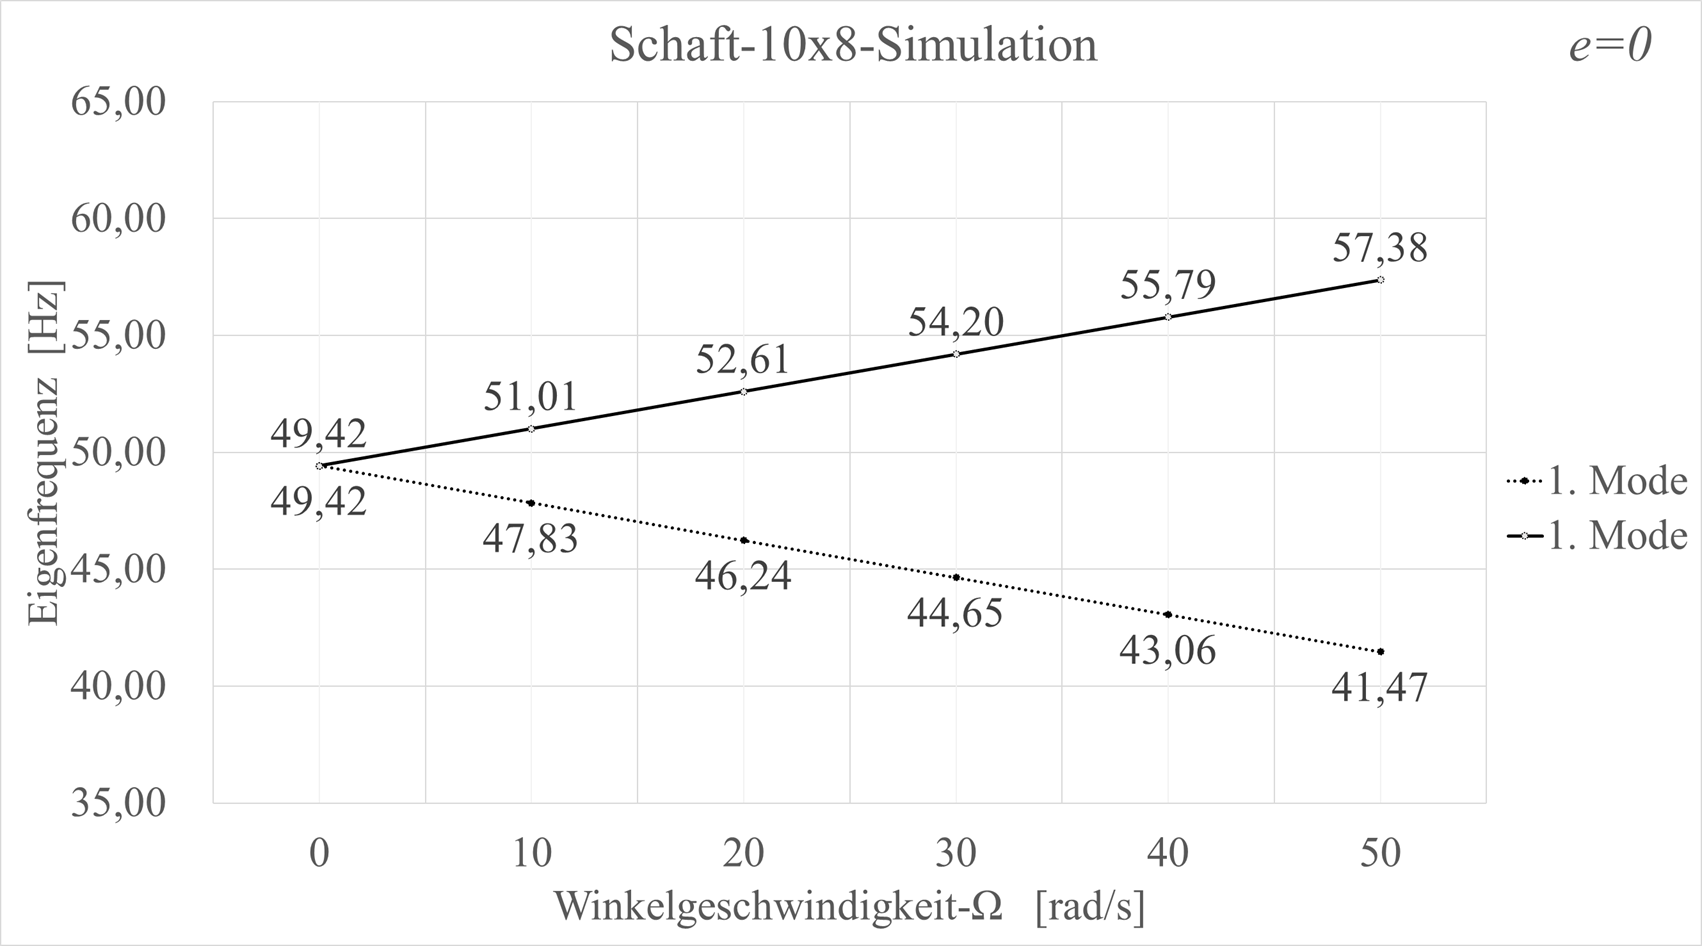
\includegraphics[width=0.95\linewidth, height=0.35\textheight]{Ergebnisse/Schaft_10x8_1Mode_Simu}
		\caption{Eigenfrequenzen vom 1. Biegemode in Abhängigkeit der Winkelgeschwindigkeit bei einem Exzentrizitätsfehler von $ e=0 $. Berechnungsparameter: Schaft $ 10\times8 $, $\rho = 7800 \,\text{kg}/\text{m}^{3} $, $ E=2,1\cdot 10^{11} \,\text{N}/\text{m}^{2} $, $ \nu=0,28 $.}
		\label{fig:Result-Schaft-10x8-Simulation-1-Mode}
	\end{figure}

	\begin{figure}[H]
		\centering
		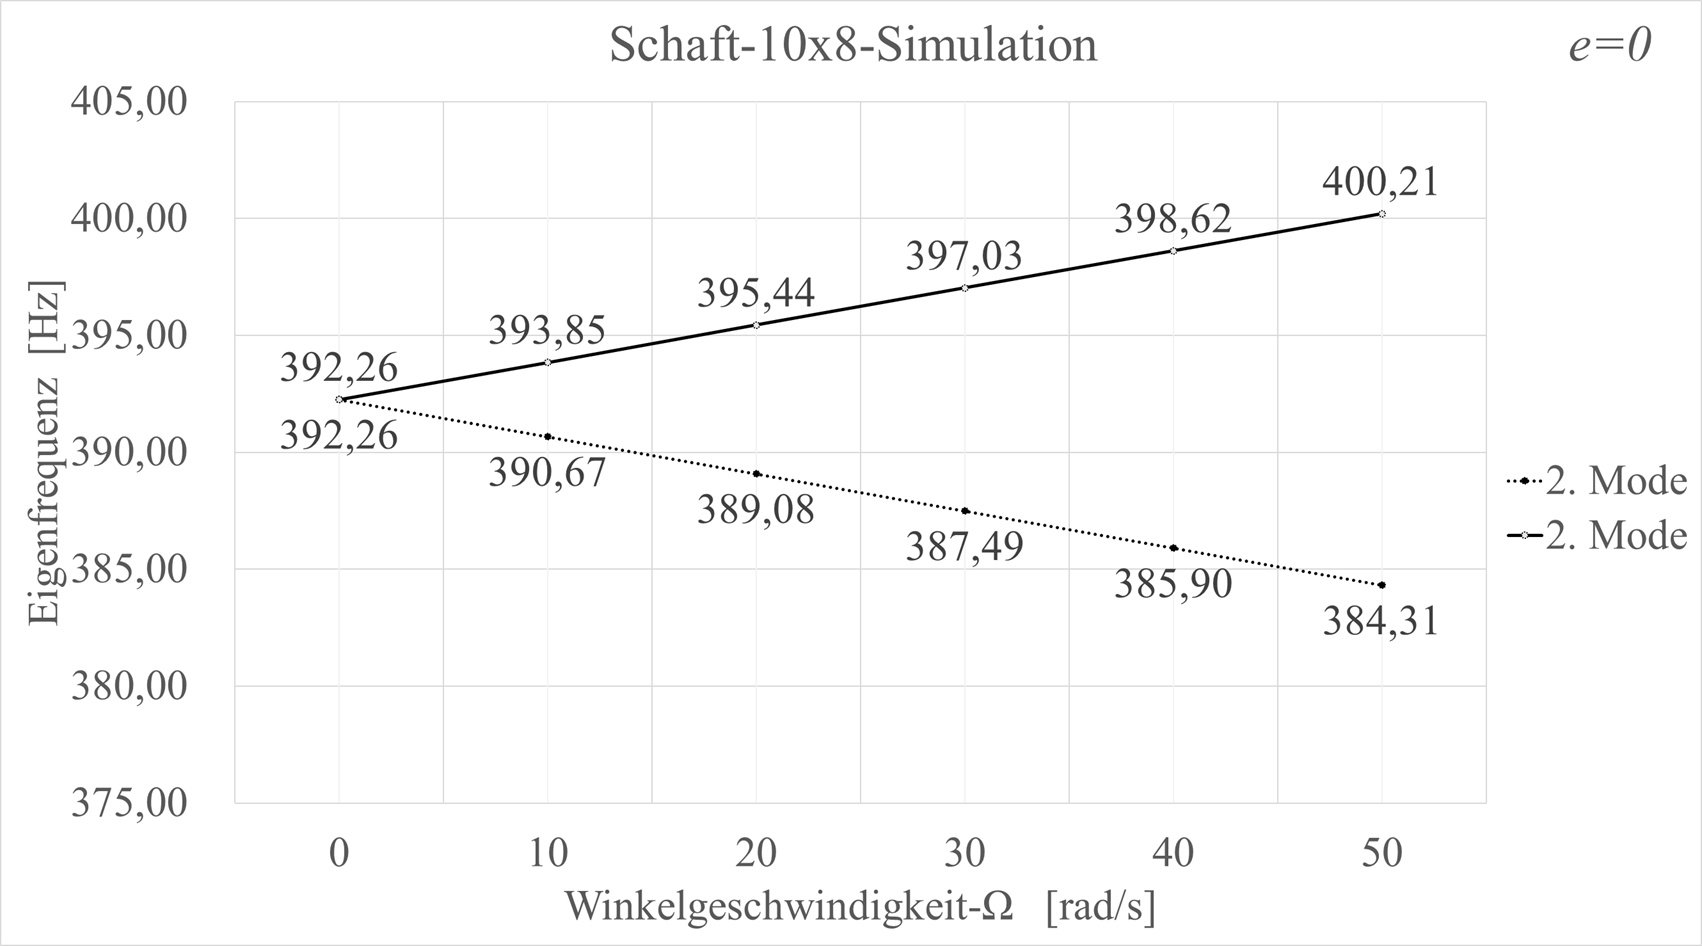
\includegraphics[width=0.95\linewidth, height=0.36\textheight]{Ergebnisse/Schaft_10x8_2Mode_Simu}
		\caption{Eigenfrequenzen vom 2. Biegemode in Abhängigkeit der Winkelgeschwindigkeit bei einem Exzentrizitätsfehler von $ e=0 $. Berechnungsparameter: Schaft $ 10\times8 $, $\rho = 7800 \,\text{kg}/\text{m}^{3} $, $ E=2,1\cdot 10^{11} \,\text{N}/\text{m}^{2} $, $ \nu=0,28 $.}
		\label{fig:Result-Schaft-10x8-Simulation-2-Mode}
	\end{figure}

	\begin{figure}[H]
		\centering
		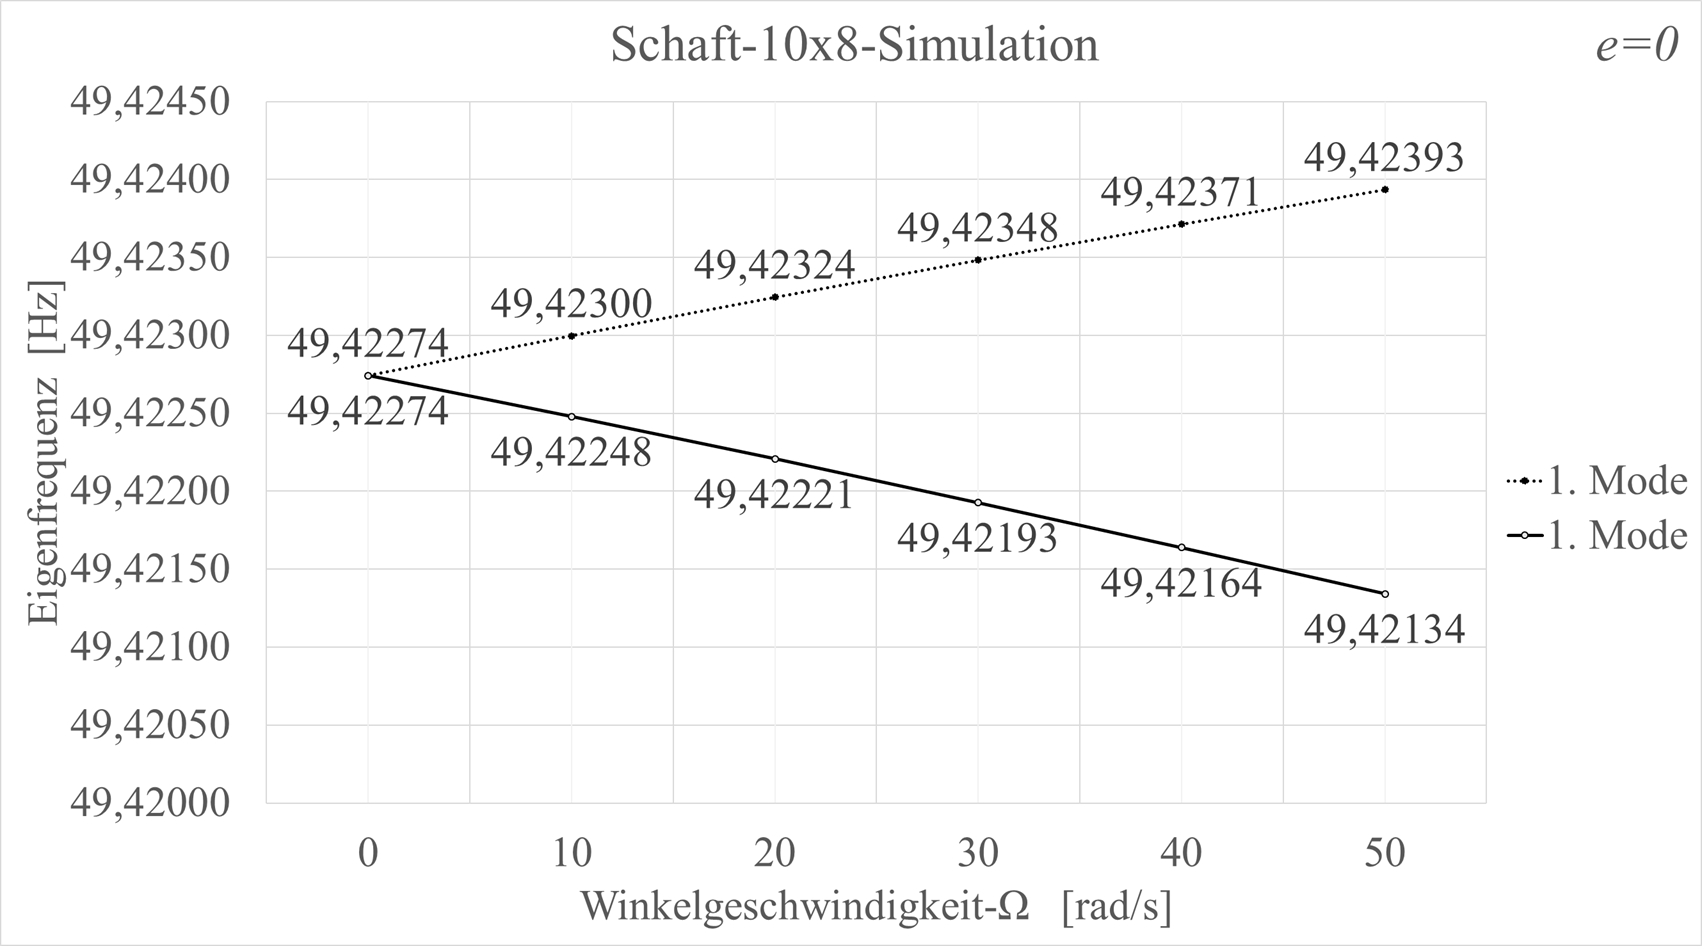
\includegraphics[width=0.95\linewidth, height=0.36\textheight]{Ergebnisse/Schaft_10x8_1Mode_Simu_ruhend}
		\caption{Eigenfrequenzen vom 1. Biegemode in Abhängigkeit der Winkelgeschwindigkeit bei einem Exzentrizitätsfehler von $ e=0 $ im ruhenden Inertialsystem. Berechnungsparameter: Schaft $ 10\times8 $, $\rho = 7800 \,\text{kg}/\text{m}^{3} $, $ E=2,1\cdot 10^{11} \,\text{N}/\text{m}^{2} $, $ \nu=0,28 $.}
		\label{fig:Result-Schaft-10x8-Simulation-1-Mode-ruhend}
	\end{figure}

	\begin{figure}[H]
		\centering
		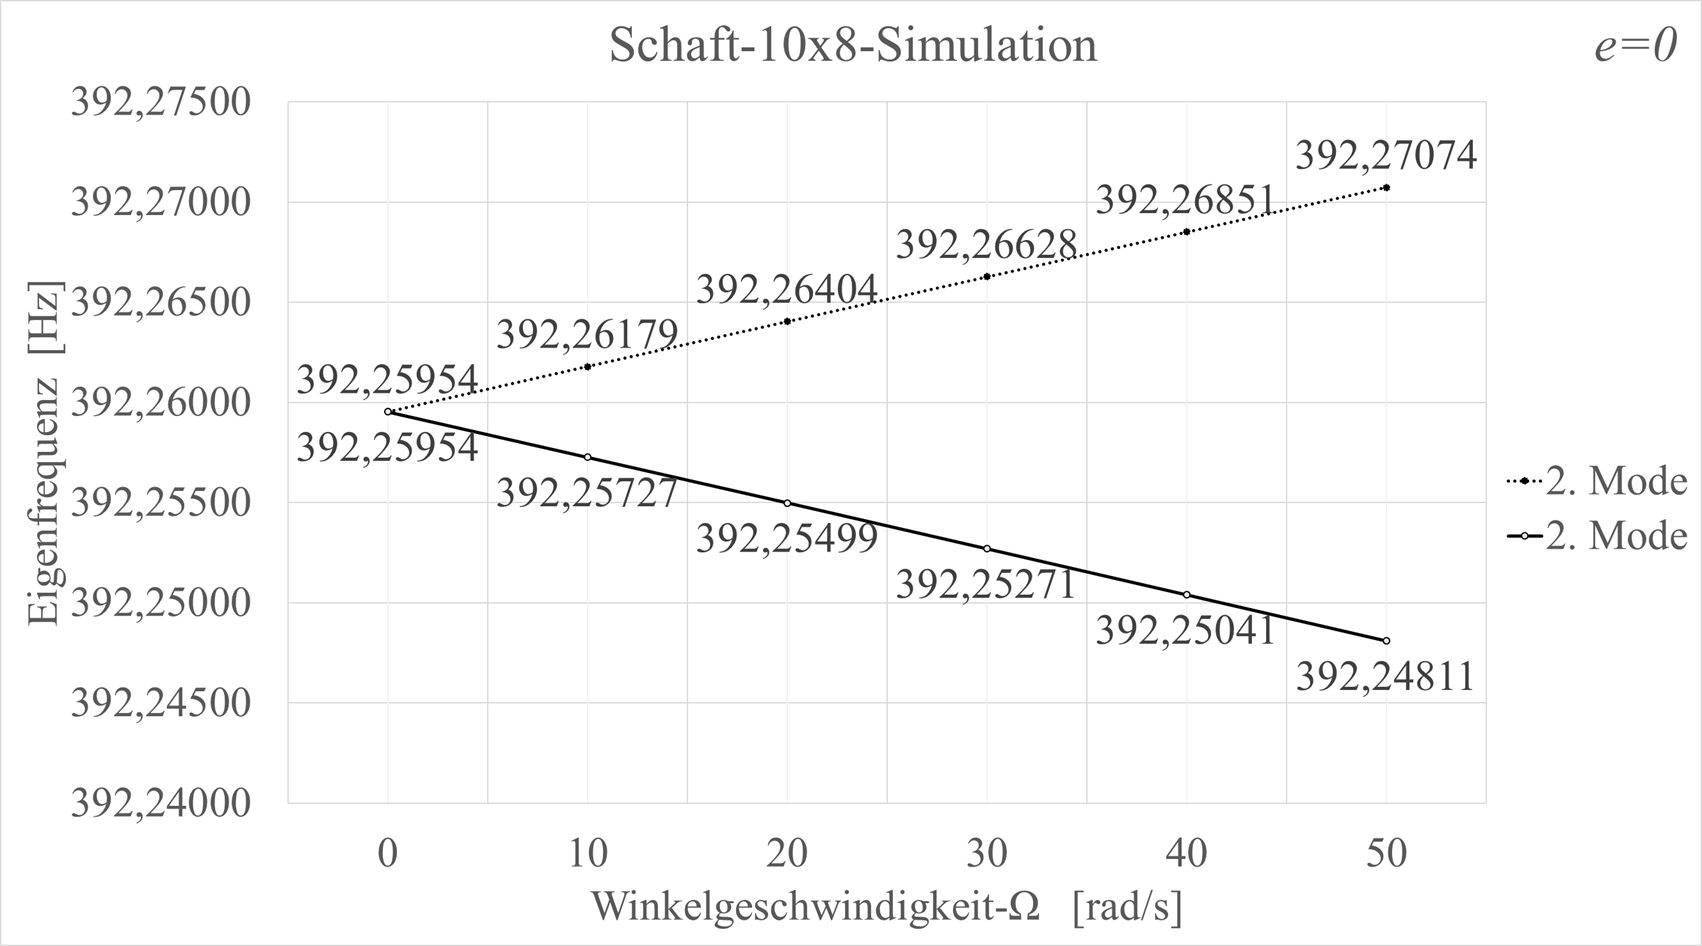
\includegraphics[width=0.95\linewidth, height=0.36\textheight]{Ergebnisse/Schaft_10x8_2Mode_Simu_ruhend}
		\caption{Eigenfrequenzen vom 2. Biegemode in Abhängigkeit der Winkelgeschwindigkeit bei einem Exzentrizitätsfehler von $ e=0 $ im ruhenden Inertialsystem. Berechnungsparameter: Schaft $ 10\times8 $, $\rho = 7800 \,\text{kg}/\text{m}^{3} $, $ E=2,1\cdot 10^{11} \,\text{N}/\text{m}^{2} $, $ \nu=0,28 $.}
		\label{fig:Result-Schaft-10x8-Simulation-2-Mode-ruhend}
	\end{figure}
	
	\begin{figure}[H]
		\centering
		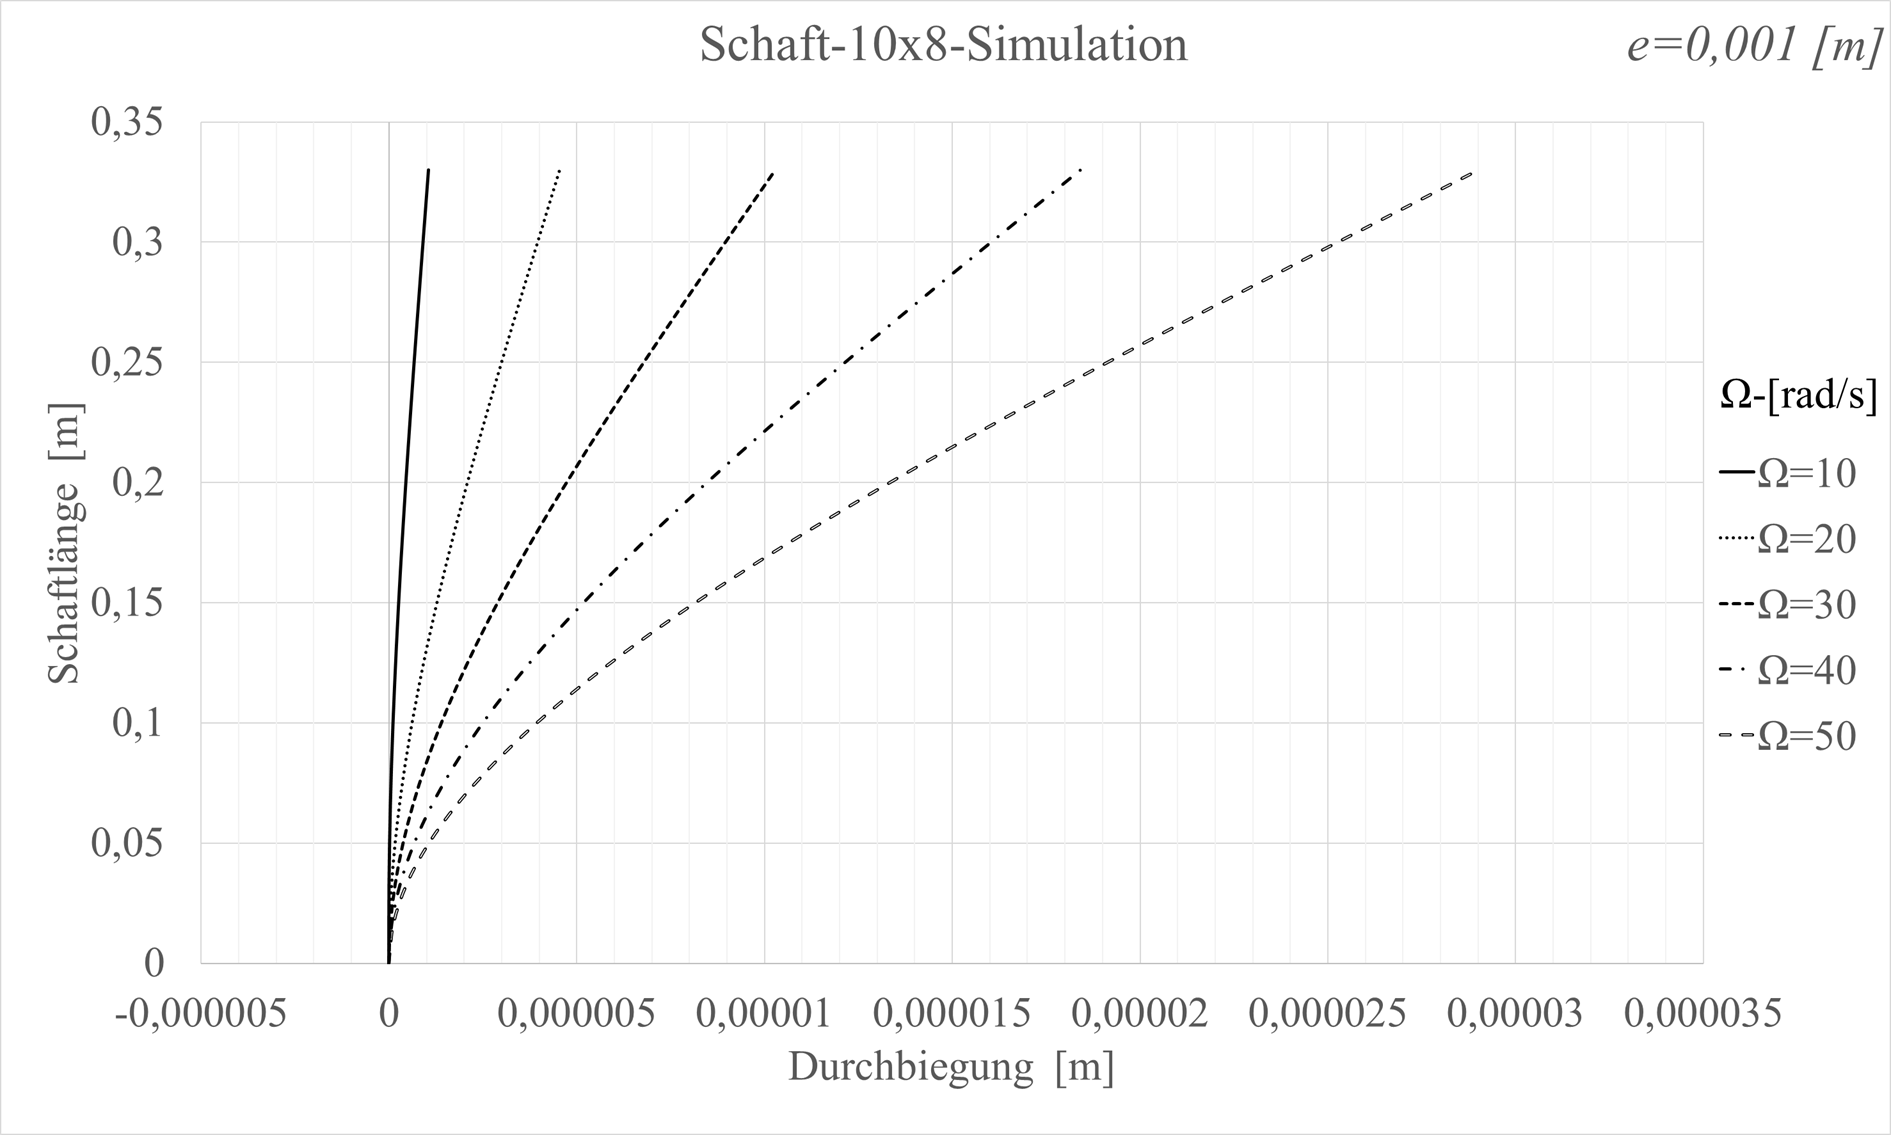
\includegraphics[width=0.95\linewidth, height=0.40\textheight]{Ergebnisse/Schaft_10x8_Biegung_Simu} 
		\caption{Durchbiegung in Abhängigkeit der Winkelgeschwindigkeit bei einem Exzentrizitätsfehler von $ e=0,001\,\text{m}$. Berechnungsparameter: Schaft $ 10\times8 $, $\rho = 7800 \,\text{kg}/\text{m}^{3} $, $ E=2,1\cdot 10^{11} \,\text{N}/\text{m}^{2} $, $ \nu=0,28 $.}
		\label{fig:Result-Schaft-10x8-Simulation-Durchbiegung}
	\end{figure}

	
	\begin{figure}[H]
		\centering
		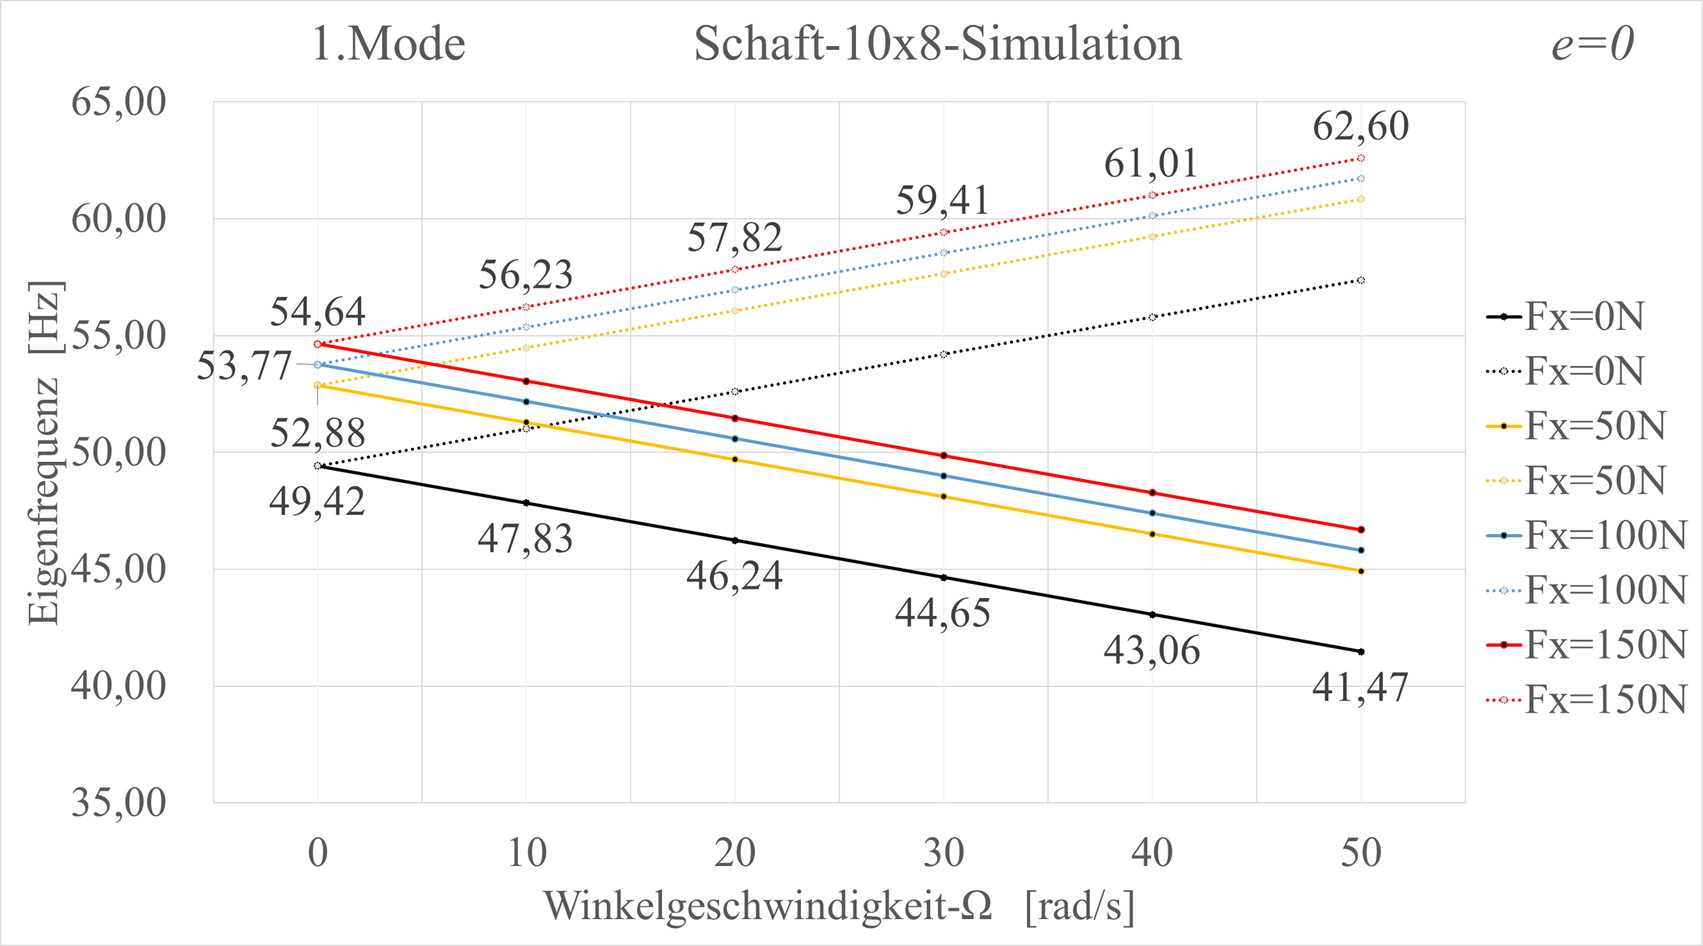
\includegraphics[width=0.93\linewidth, height=0.33\textheight]{Ergebnisse/Schaft_10x8_Zugkraft_Simu} 
		\caption{Eigenfrequenzen vom 1. Biegemode in Abhängigkeit der Winkelgeschwindigkeit $ \Omega $ und der Zugkraft $ Fx $ bei bei einem Exzentrizitätsfehler von $ e=0 $. Berechnungsparameter: Schaft $ 10\times8 $, $\rho = 7800 \,\text{kg}/\text{m}^{3} $, $ E=2,1\cdot 10^{11} \,\text{N}/\text{m}^{2} $, $ \nu=0,28 $.}
		\label{fig:Result-Schaft-10x8-Simulation-Zugkraft}
	\end{figure}
	
	Die experimentellen Ergebnissen werden gemäß den verschiedenen Messrichtungen des Beschleunigungssensors in die zwei Fälle unterteilt. Die Messrichtung erfolgt entweder parallel oder senkrecht zur Anregungsrichtung. Nach Gleichung \ref{equ:Verhältnis-Rotaion-und-Radialkraft} kann die Radialkraft in ein Produkt aus Exzentrizitätsfehler ($ e=0,001\,\text{m}$) und Winkelgeschwindigkeit umgerechnet werden. Weitere experimentelle Ergebnisse sind in den Abbildungen \ref{fig:Result-Schaft-10x8-1Mode-Ver1} bis \ref{fig:Result-Schaft-10x8-2Mode-Ver3} dargestellt.
	
	\begin{figure}[H]
		\centering
		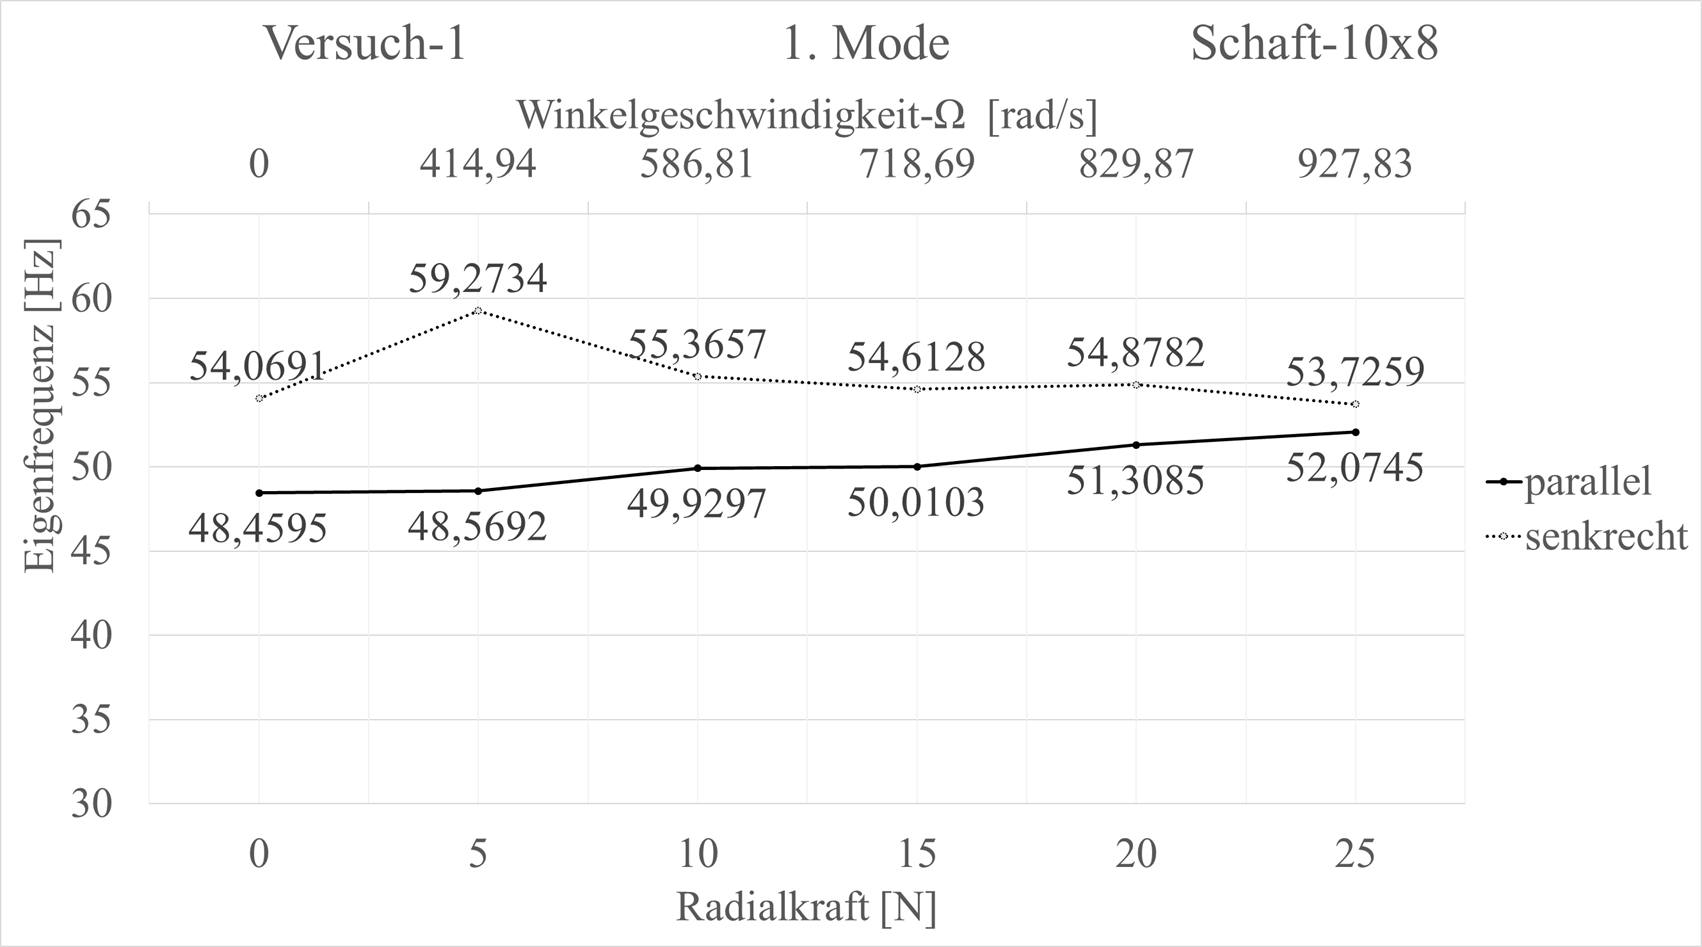
\includegraphics[width=0.93\linewidth, height=0.33\textheight]{Ergebnisse/Schaft_10x8_1Mode_ver1} 
		\caption{Gemessene Eigenfrequenzen vom 1. Biegemode in Abhängigkeit der Vorspannkraft. Angabe der Eigenfrequenzen parallel und senkrecht zur Vorspannrichtung. (Probe Nr. 1 (Schaft $ 10\times8 $ ), Versuchsreihe 1)}
		\label{fig:Result-Schaft-10x8-1Mode-Ver1}
	\end{figure}

	\begin{figure}[H]
		\centering
		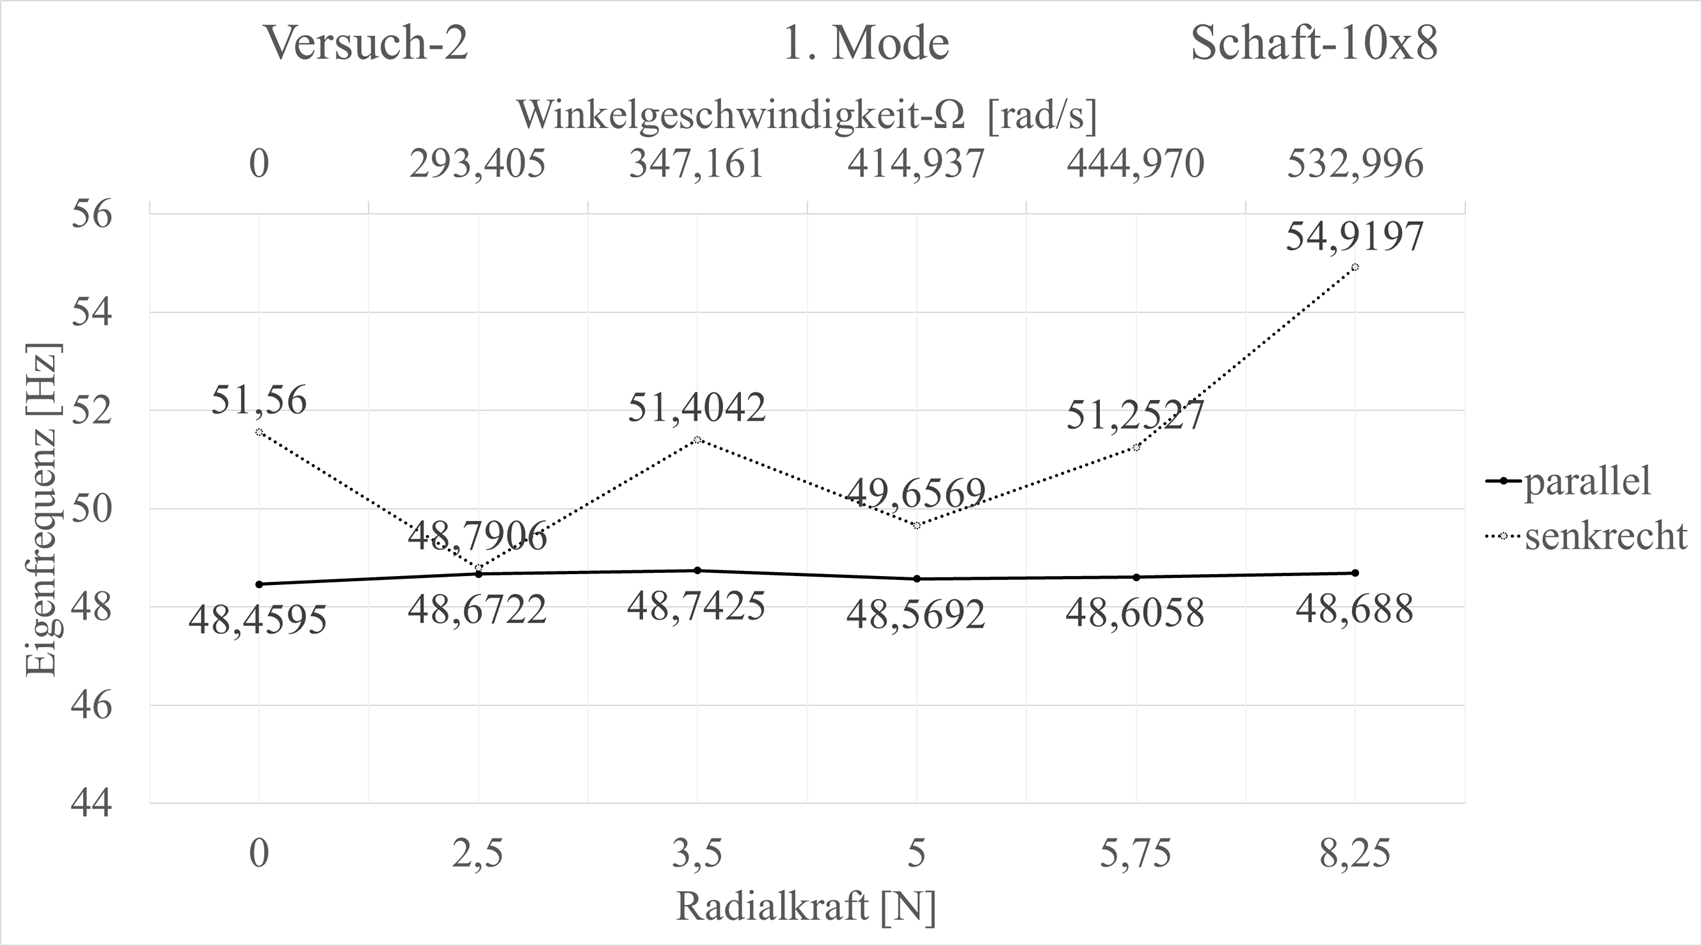
\includegraphics[width=0.95\linewidth, height=0.36\textheight]{Ergebnisse/Schaft_10x8_1Mode_ver2}
		\caption{Gemessene Eigenfrequenzen vom 1. Biegemode in Abhängigkeit der Vorspannkraft. Angabe der Eigenfrequenzen parallel und senkrecht zur Vorspannrichtung (Probe Nr. 1 (Schaft $ 10\times8 $ ), Versuchsreihe 2).}
		\label{fig:Result-Schaft-10x8-1Mode-Ver2}
	\end{figure}

	\begin{figure}[H]
		\centering
		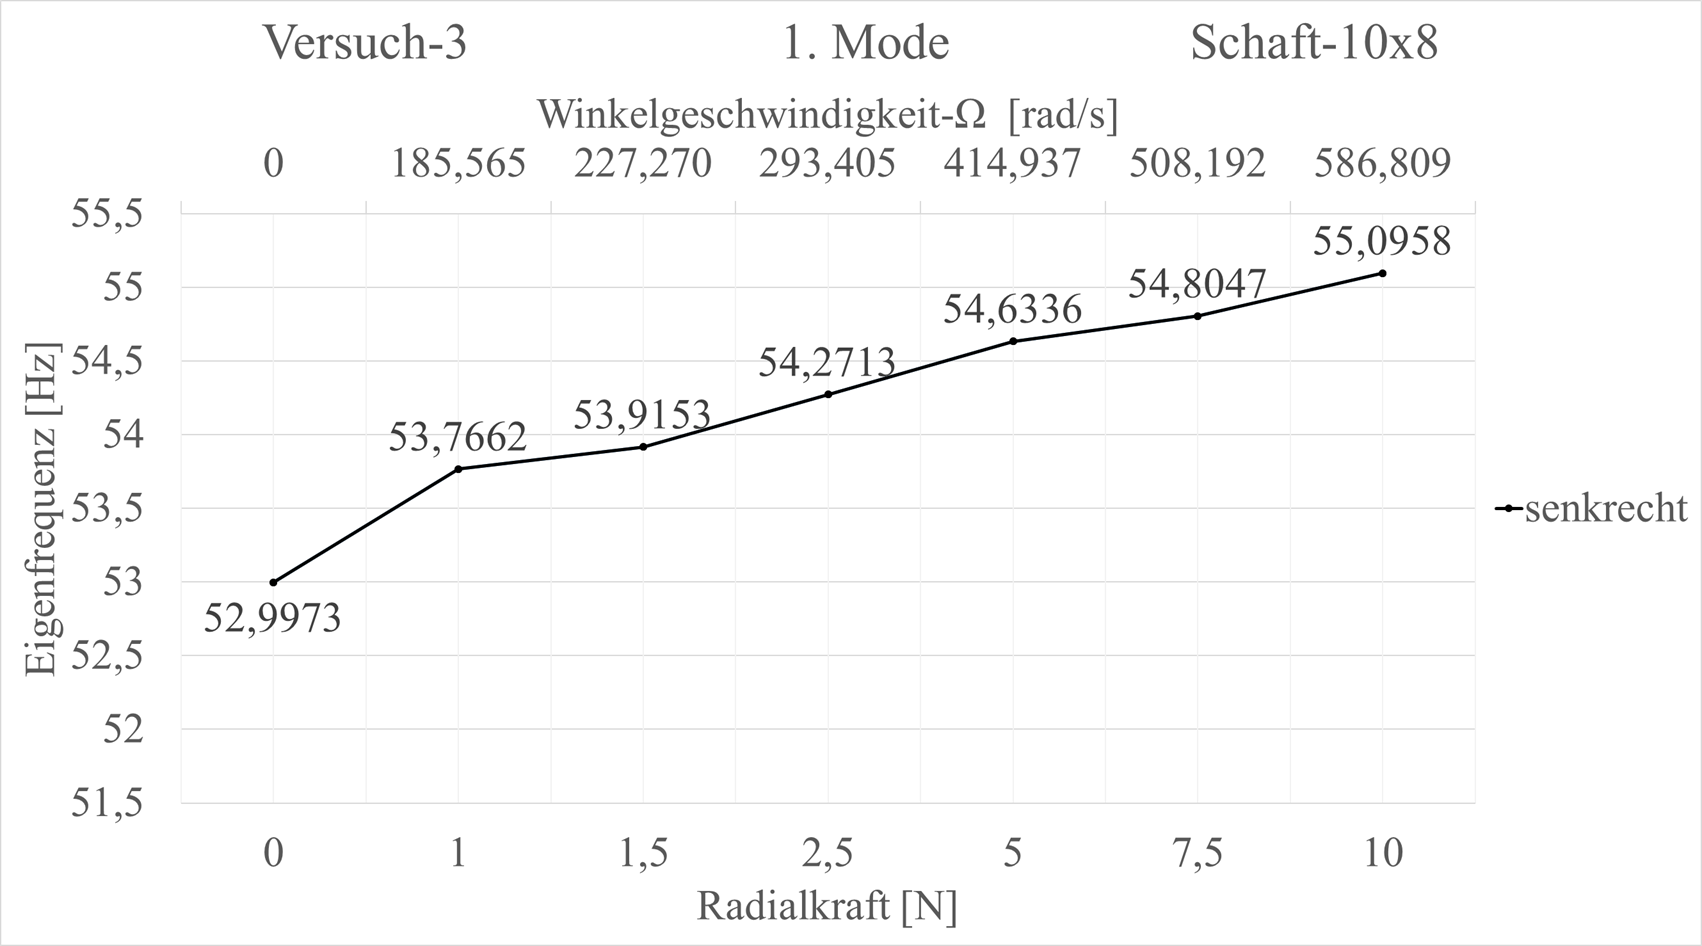
\includegraphics[width=0.95\linewidth, height=0.36\textheight]{Ergebnisse/Schaft_10x8_1Mode_ver3}
		\caption{Gemessene Eigenfrequenzen vom 1. Biegemode in Abhängigkeit der Vorspannkraft. Angabe der Eigenfrequenzen senkrecht zur Vorspannrichtung (Probe Nr. 1 (Schaft $ 10\times8 $), Versuchsreihe 3).}
		\label{fig:Result-Schaft-10x8-1Mode-Ver3}
	\end{figure}

	\begin{figure}[H]
		\centering
		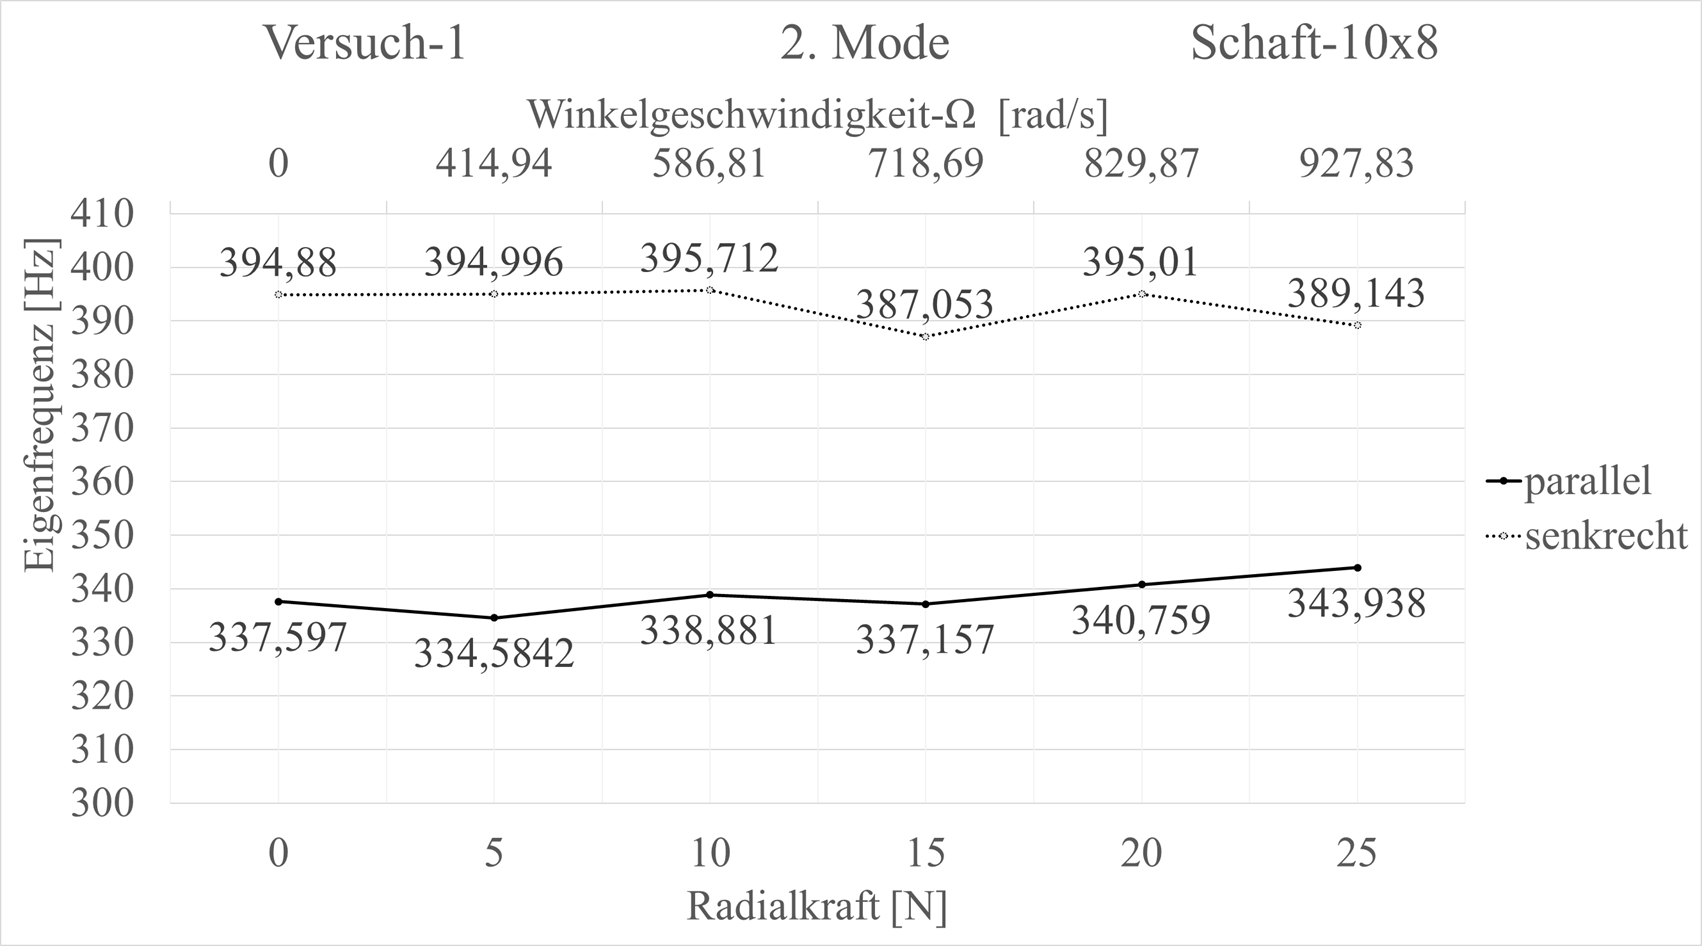
\includegraphics[width=0.95\linewidth, height=0.36\textheight]{Ergebnisse/Schaft_10x8_2Mode_ver1} 
		\caption{Gemessene Eigenfrequenzen vom 2. Biegemode in Abhängigkeit der Vorspannkraft. Angabe der Eigenfrequenzen parallel und senkrecht zur Vorspannrichtung (Probe Nr. 1 (Schaft $ 10\times8 $ ), Versuchsreihe 1).}
		\label{fig:Result-Schaft-10x8-2Mode-Ver1}
	\end{figure}

	\begin{figure}[H]
		\centering
		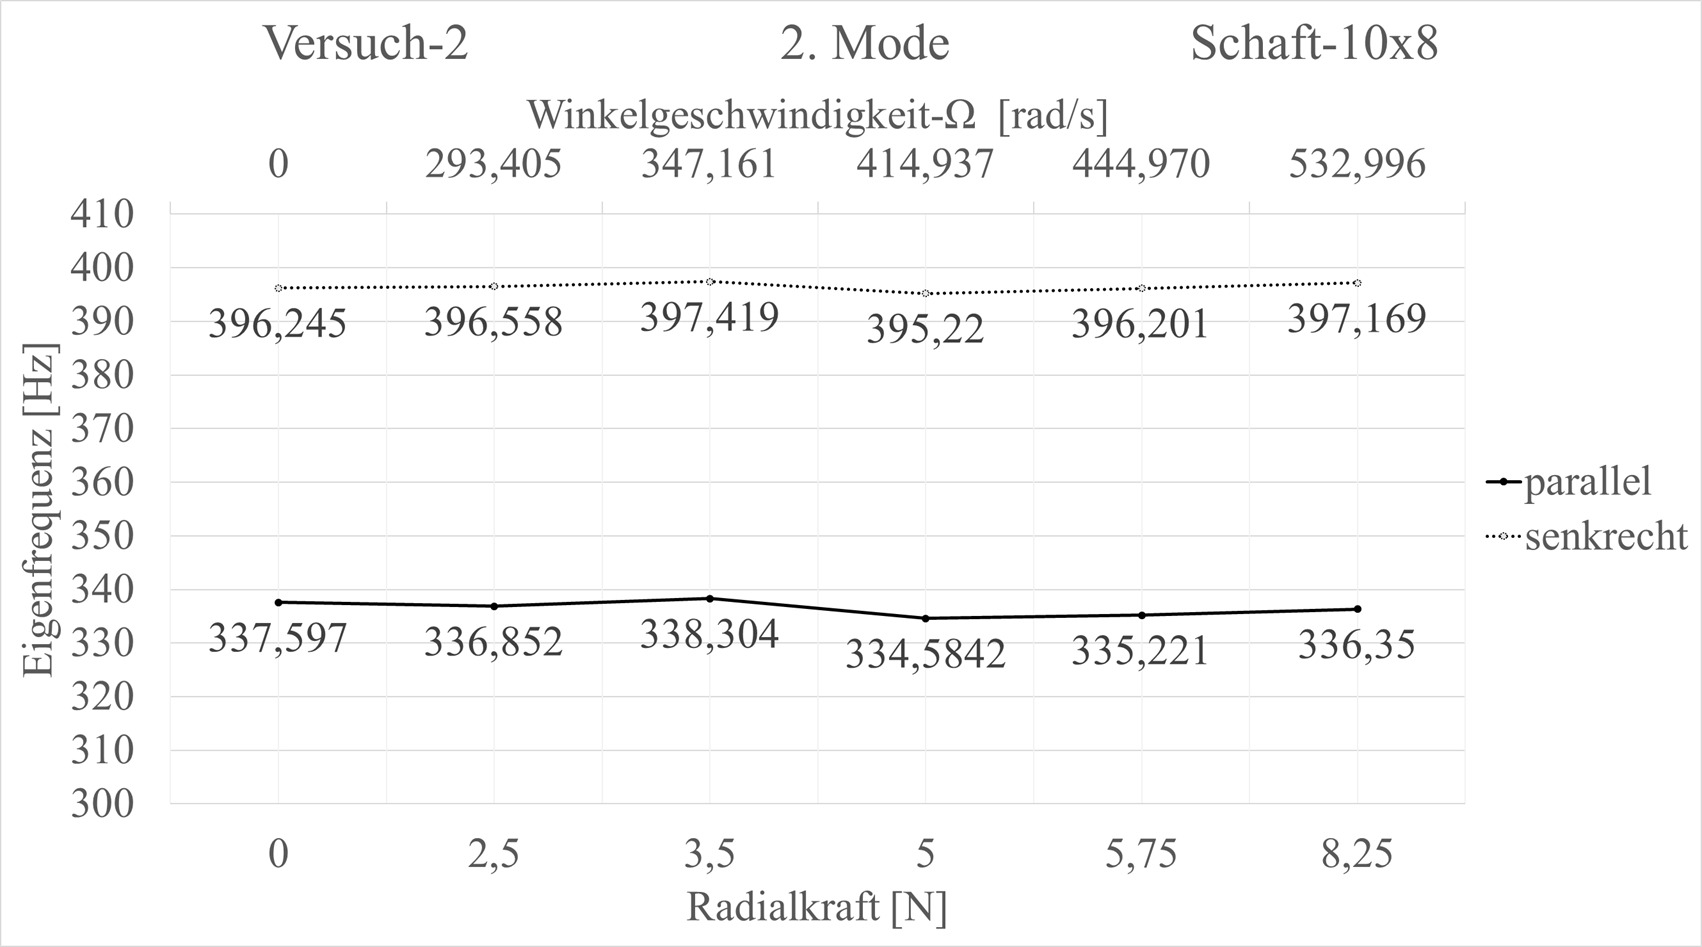
\includegraphics[width=0.95\linewidth, height=0.36\textheight]{Ergebnisse/Schaft_10x8_2Mode_ver2}
		\caption{Gemessene Eigenfrequenzen vom 1. Biegemode in Abhängigkeit der Vorspannkraft. Angabe der Eigenfrequenzen parallel und senkrecht zur Vorspannrichtung (Probe Nr. 1 (Schaft $ 10\times8 $ ), Versuchsreihe 2).}
		\label{fig:Result-Schaft-10x8-2Mode-Ver2}
	\end{figure}

	\begin{figure}[H]
		\centering
		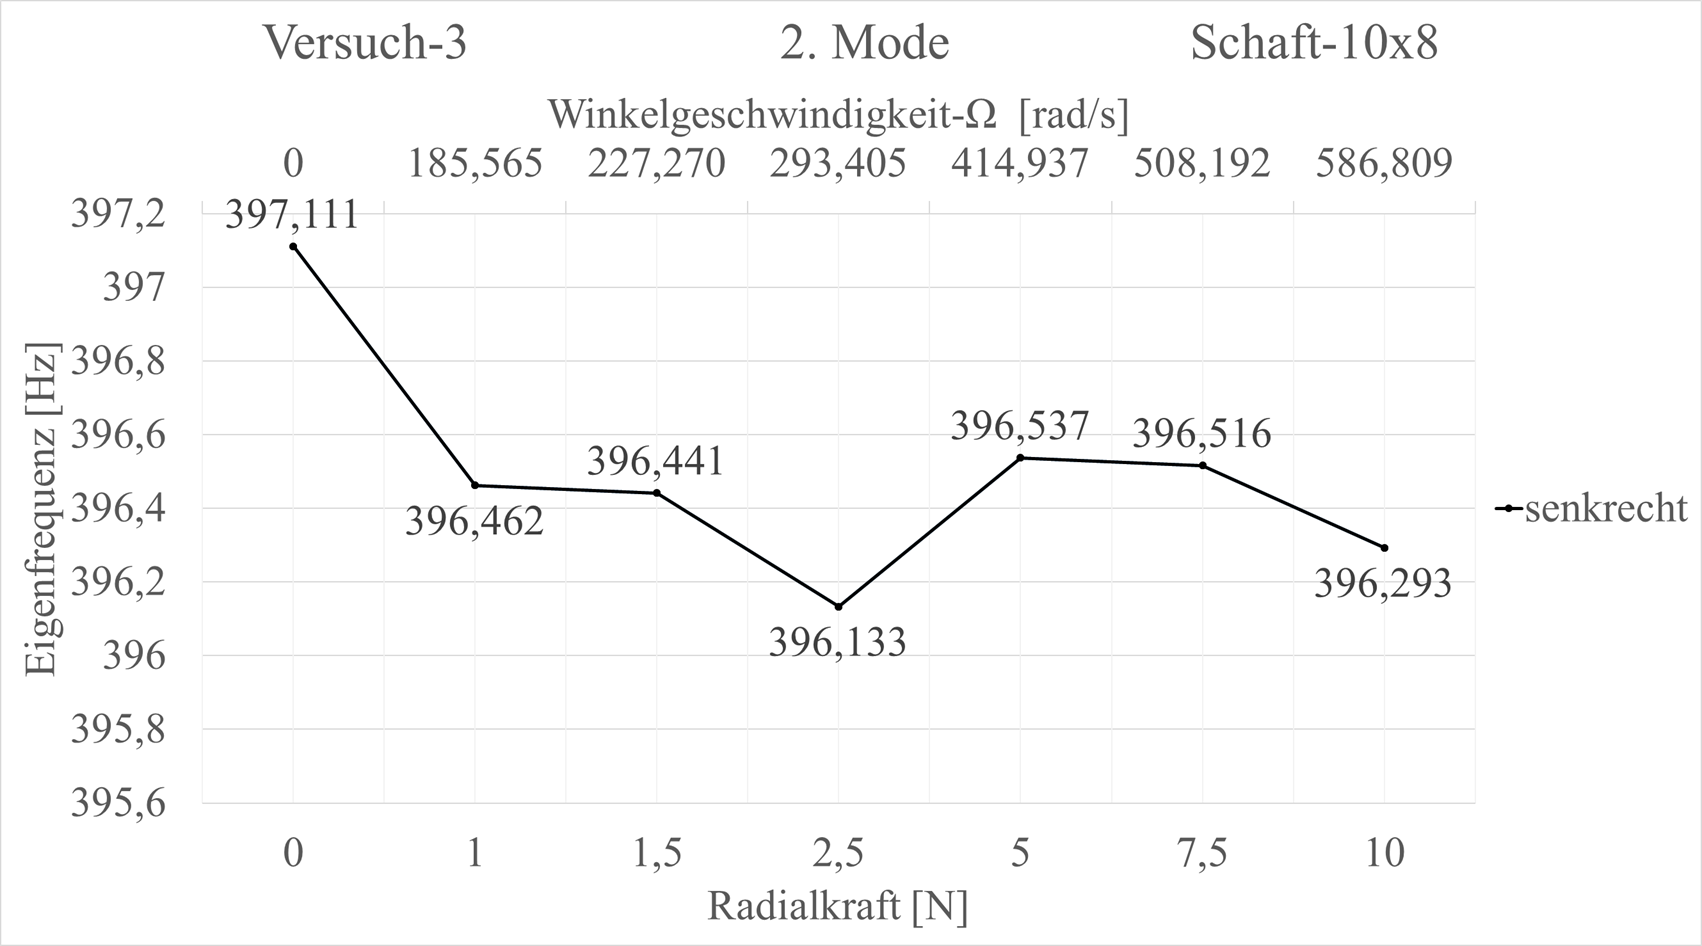
\includegraphics[width=0.95\linewidth, height=0.36\textheight]{Ergebnisse/Schaft_10x8_2Mode_ver3}
		\caption{Gemessene Eigenfrequenzen vom 1. Biegemode in Abhängigkeit der Vorspannkraft. Angabe der Eigenfrequenzen senkrecht zur Vorspannrichtung (Probe Nr. 1 (Schaft $ 10\times8 $), Versuchsreihe 3).}
		\label{fig:Result-Schaft-10x8-2Mode-Ver3}
	\end{figure}
	
	Die Abbildungen \ref{fig:Result-Schaft-10x8-1Mode-Ver1} bis \ref{fig:Result-Schaft-10x8-1Mode-Ver3} zeigen die Ergebnisse für die ersten beiden Moden. Eine klare Abhängigkeit der Eigenfrequenzen lässt sich nur schwer ableiten. Tendenziell nehmen die Eigenfrequenzen senkrecht zur Vorspannrichtung mit zunehmender Vorspannkraft leicht zu (vgl. Abbildung \ref{fig:Result-Schaft-10x8-1Mode-Ver2} und \ref{fig:Result-Schaft-10x8-1Mode-Ver3}). Parallel zur Vorspannrichtung ist der Einfluss der Vorspannkraft auf die Eigenfrequenzen geringer. Die Ungenauigkeiten der experimentellen Ergebnisse begründen sich mit verschiedenen Störungen und Messungenauigkeiten. Die Eigenfrequenz des ersten Modes im senkrechten Fall zeigt, dass mit zunehmender Radialkraft die Eigenfrequenz allmählich zunimmt. Werden die gemessenen und berechneten Eigenfrequenzen für den ruhenden Schaft verglichen, so fällt auf, dass die gemessenen Werte niedriger sind. Ursache dafür sind die zusätzliche Massen durch den Beschleunigungssensor und die Feder. 
	
	
	\subsection{Probe Nr. 2 (Schaft 10$\times$9)}	
	Als zweiter Probekörper wird der Schaft-$10\times9 $ betrachtet. Die Materialparameter sind identisch zu Probe Nr.1. In den Abbildungen \ref{fig:Result-Schaft-10x9-Simulation-1-Mode} bis \ref{fig:Result-Schaft-10x9-Simulation-Zugkraft} sind zunächst wieder die Simulationsergebnisse dargestellt. Die experimentellen Ergebnisse sind anschließend in den Abbildungen \ref{fig:Result-Schaft-10x9-1Mode-Ver1} bis \ref{fig:Result-Schaft-10x9-2Mode-Ver2} dargestellt.\\
	
	Der Einfluss der Winkelgeschwindigkeit $\Omega$ und der Zugkraft $ Fx $ auf die Eigenfrequenzen ist ähnlich zu den Ergebnissen für Probe 1. Weiterhin hat auch hier der Exzentrizitätsfehler in Verbindung mit einer Winkelgeschwindigkeit keinen Einfluss auf die Eigenfrequenzen. Jedoch sind die Eigenfrequenzen im ruhenden Zustand für die Probe 2 niedriger als für Probe 1. Der Einfluss der Winkelgeschwindigkeit $\Omega$ auf die Durchbiegung ist analog zu den Ergebnissen für Probe 1. Jedoch sind die Durchbiegungen für die Probe 2, wegen der geringeren Steifigkeit, größer als bei Probe 1. \\
	
	\begin{figure}[H]
		\centering
		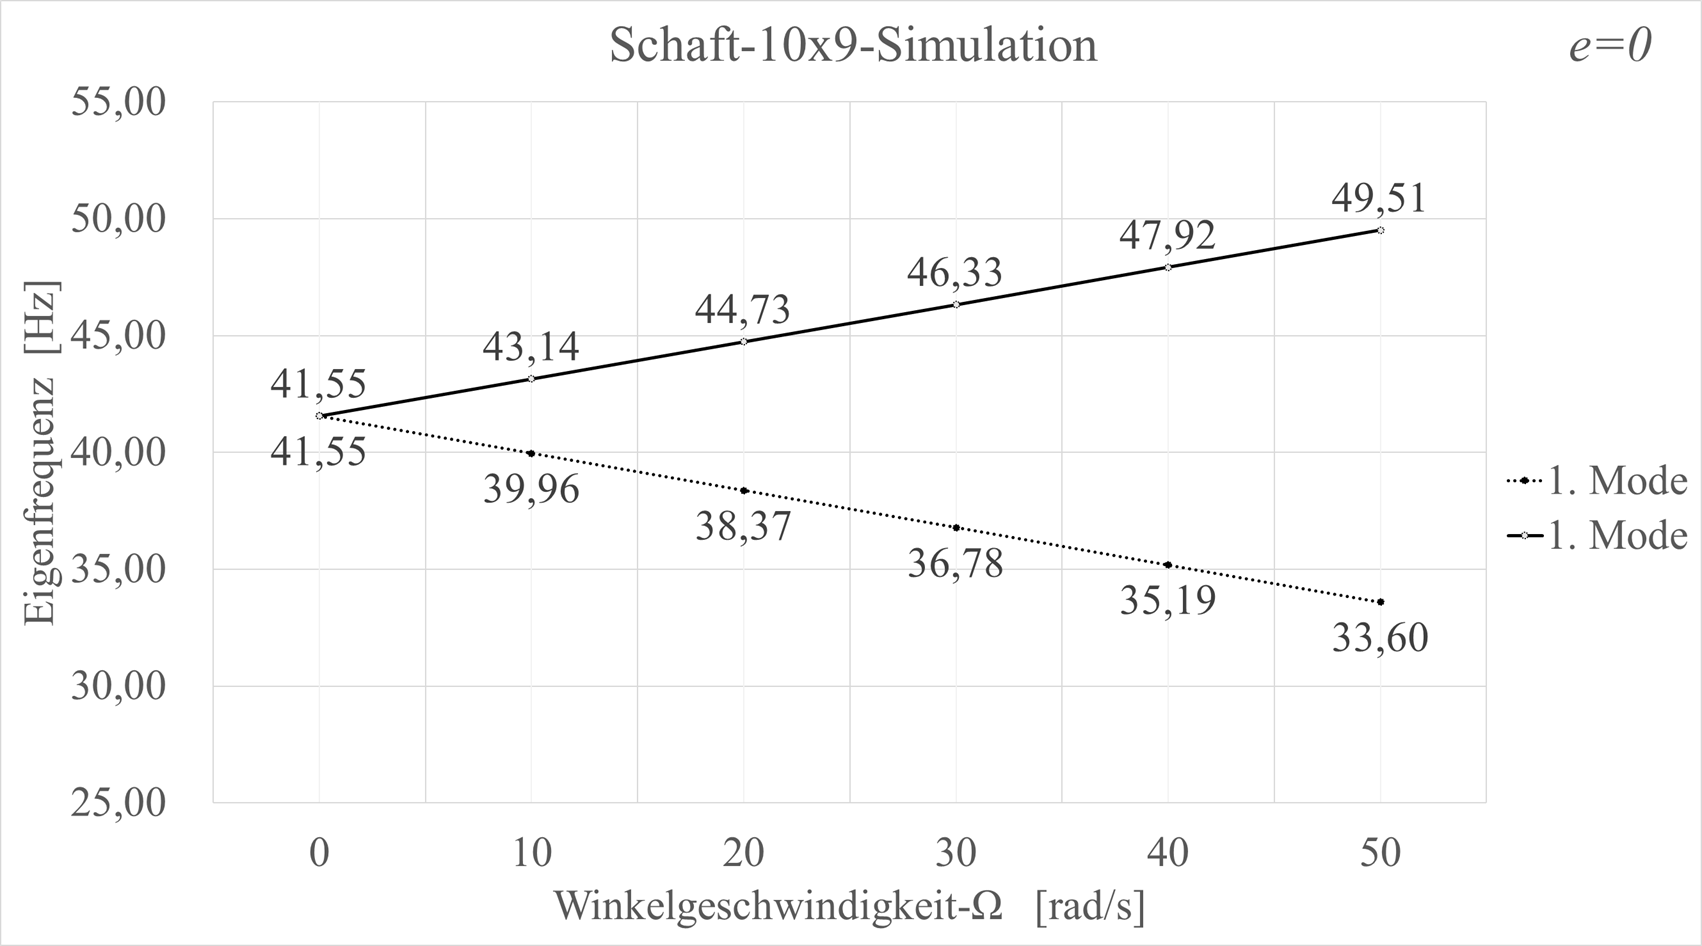
\includegraphics[width=0.95\linewidth, height=0.36\textheight]{Ergebnisse/Schaft_10x9_1Mode_Simu}
		\caption{Eigenfrequenzen vom 1. Biegemode in Abhängigkeit der Winkelgeschwindigkeit bei einem Exzentrizitätsfehler von $ e=0 $. Berechnungsparameter: Schaft $ 10\times9 $, $\rho = 7800 \,\text{kg}/\text{m}^{3} $, $ E=2,1\cdot 10^{11} \,\text{N}/\text{m}^{2} $, $ \nu=0,28 $.}
		\label{fig:Result-Schaft-10x9-Simulation-1-Mode}
	\end{figure}
	
	\begin{figure}[H]
		\centering
		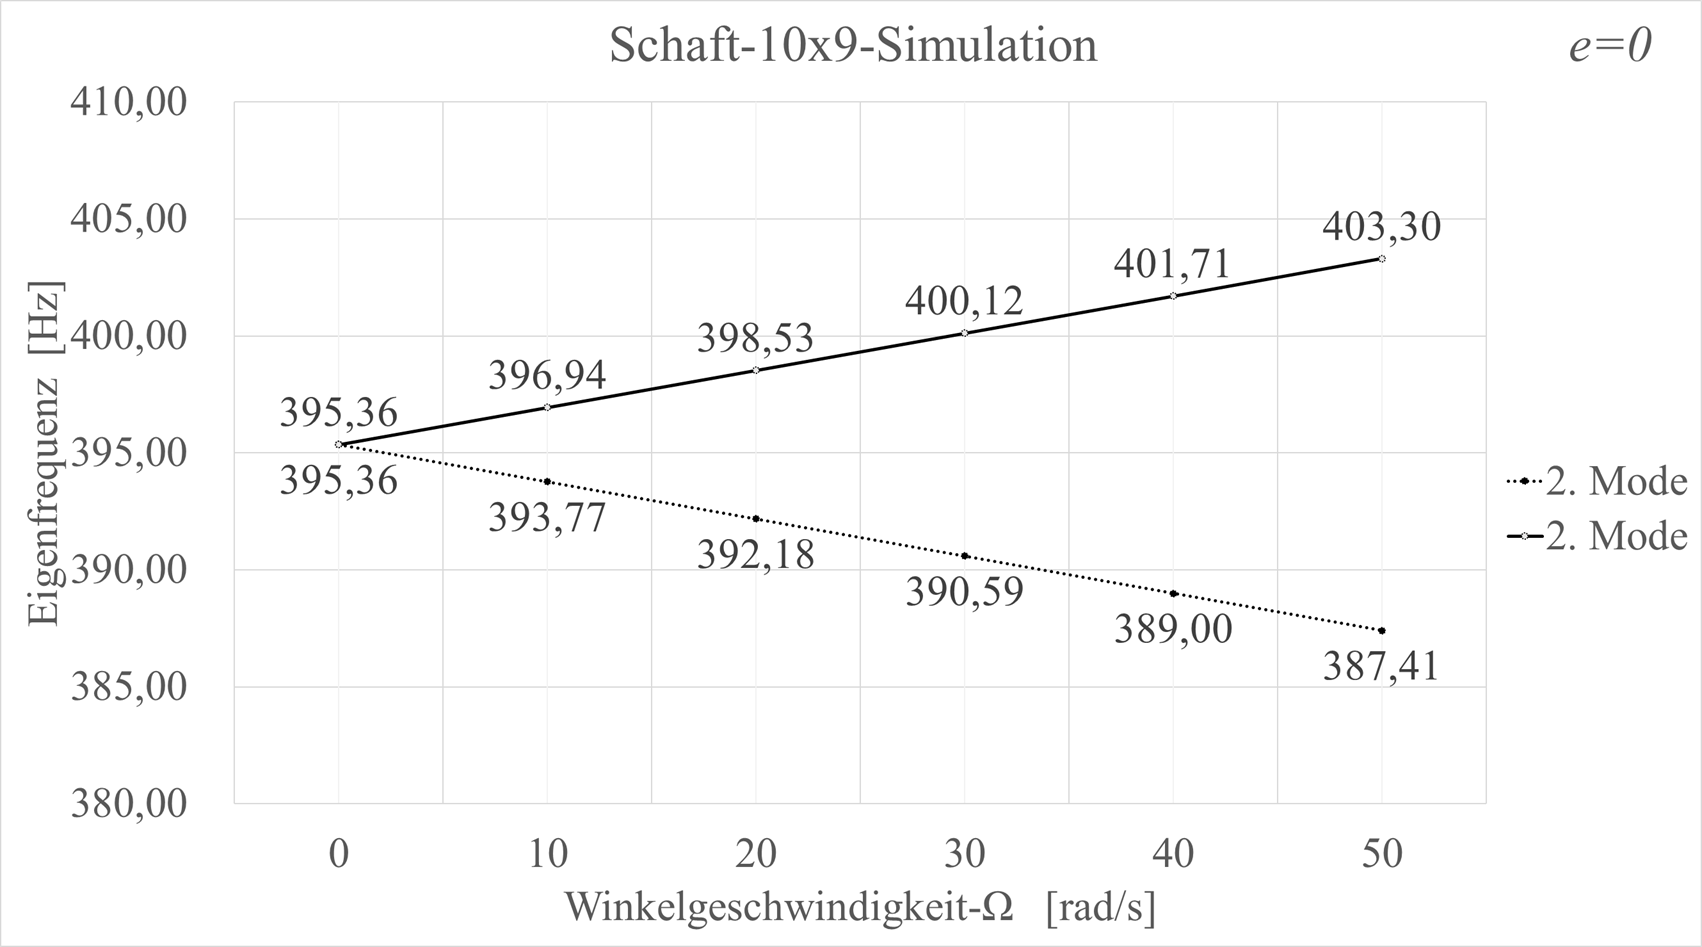
\includegraphics[width=0.95\linewidth, height=0.36\textheight]{Ergebnisse/Schaft_10x9_2Mode_Simu}
		\caption{Eigenfrequenzen vom 2. Biegemode in Abhängigkeit der Winkelgeschwindigkeit bei einem Exzentrizitätsfehler von $ e=0 $. Berechnungsparameter: Schaft $ 10\times9 $, $\rho = 7800 \,\text{kg}/\text{m}^{3} $, $ E=2,1\cdot 10^{11} \,\text{N}/\text{m}^{2} $, $ \nu=0,28 $.}
		\label{fig:Result-Schaft-10x9-Simulation-2-Mode}
	\end{figure}

	\begin{figure}[H]
		\centering
		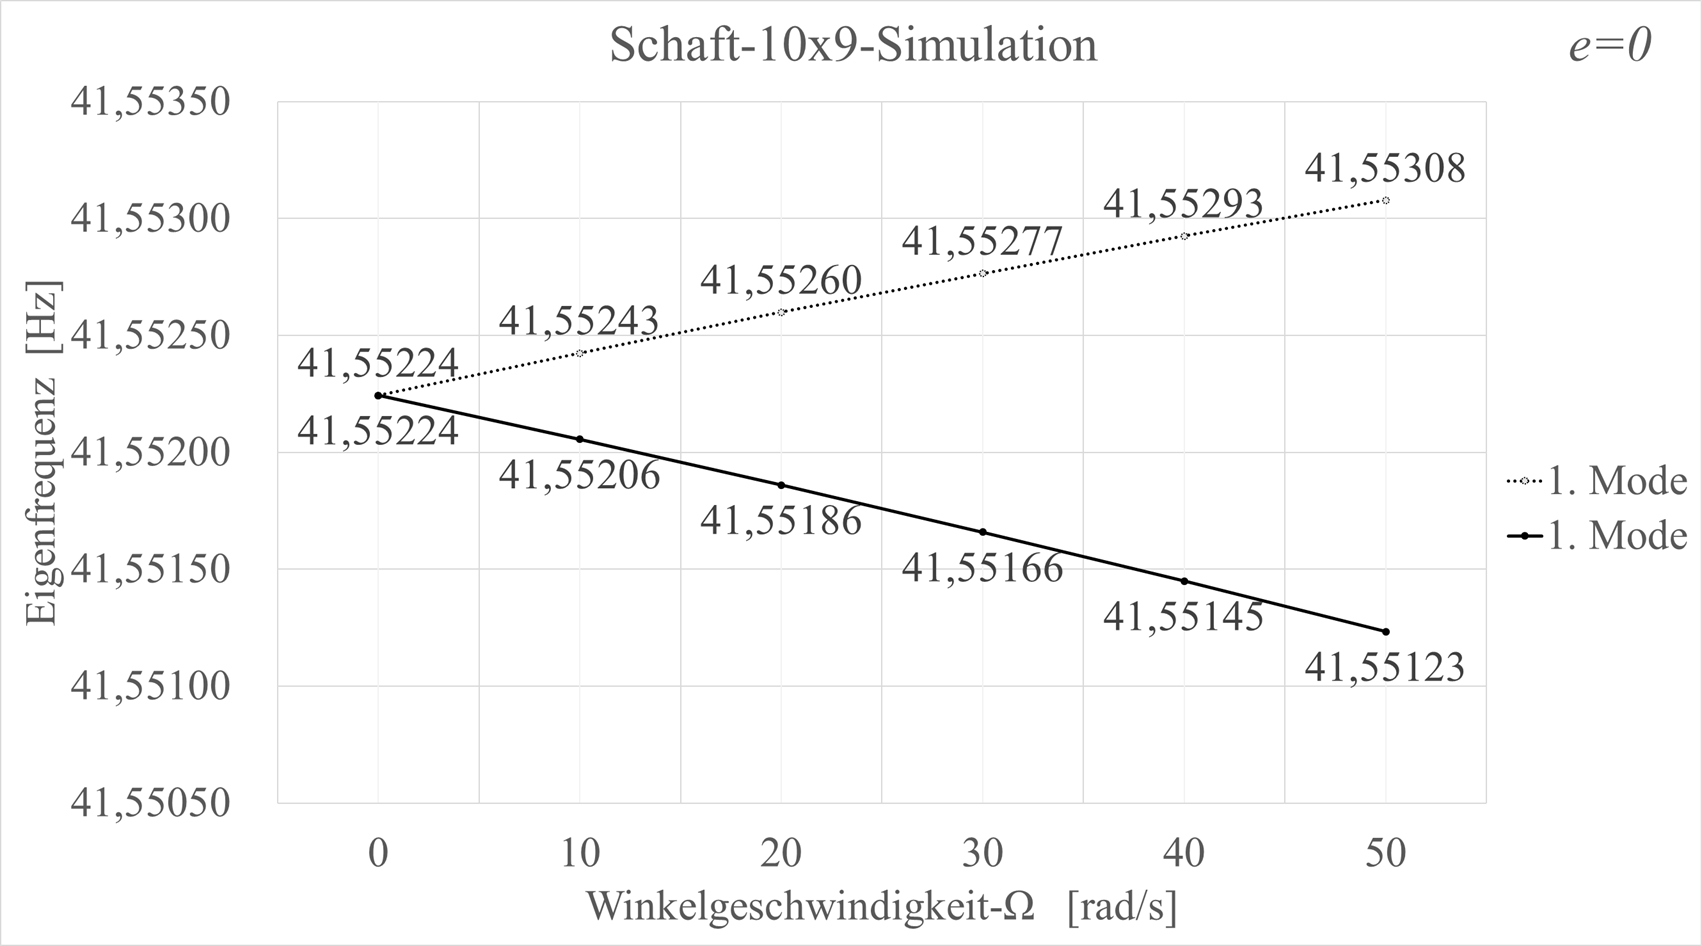
\includegraphics[width=0.95\linewidth, height=0.36\textheight]{Ergebnisse/Schaft_10x9_1Mode_Simu_ruhend}
		\caption{Eigenfrequenzen vom 1. Biegemode in Abhängigkeit der Winkelgeschwindigkeit bei einem Exzentrizitätsfehler von $ e=0 $ im ruhenden Inertialsystem. Berechnungsparameter: Schaft $ 10\times9 $, $\rho = 7800 \,\text{kg}/\text{m}^{3} $, $ E=2,1\cdot 10^{11} \,\text{N}/\text{m}^{2} $, $ \nu=0,28 $.}
		\label{fig:Result-Schaft-10x9-Simulation-1-Mode-ruhend}
	\end{figure}
	
	\begin{figure}[H]
		\centering
		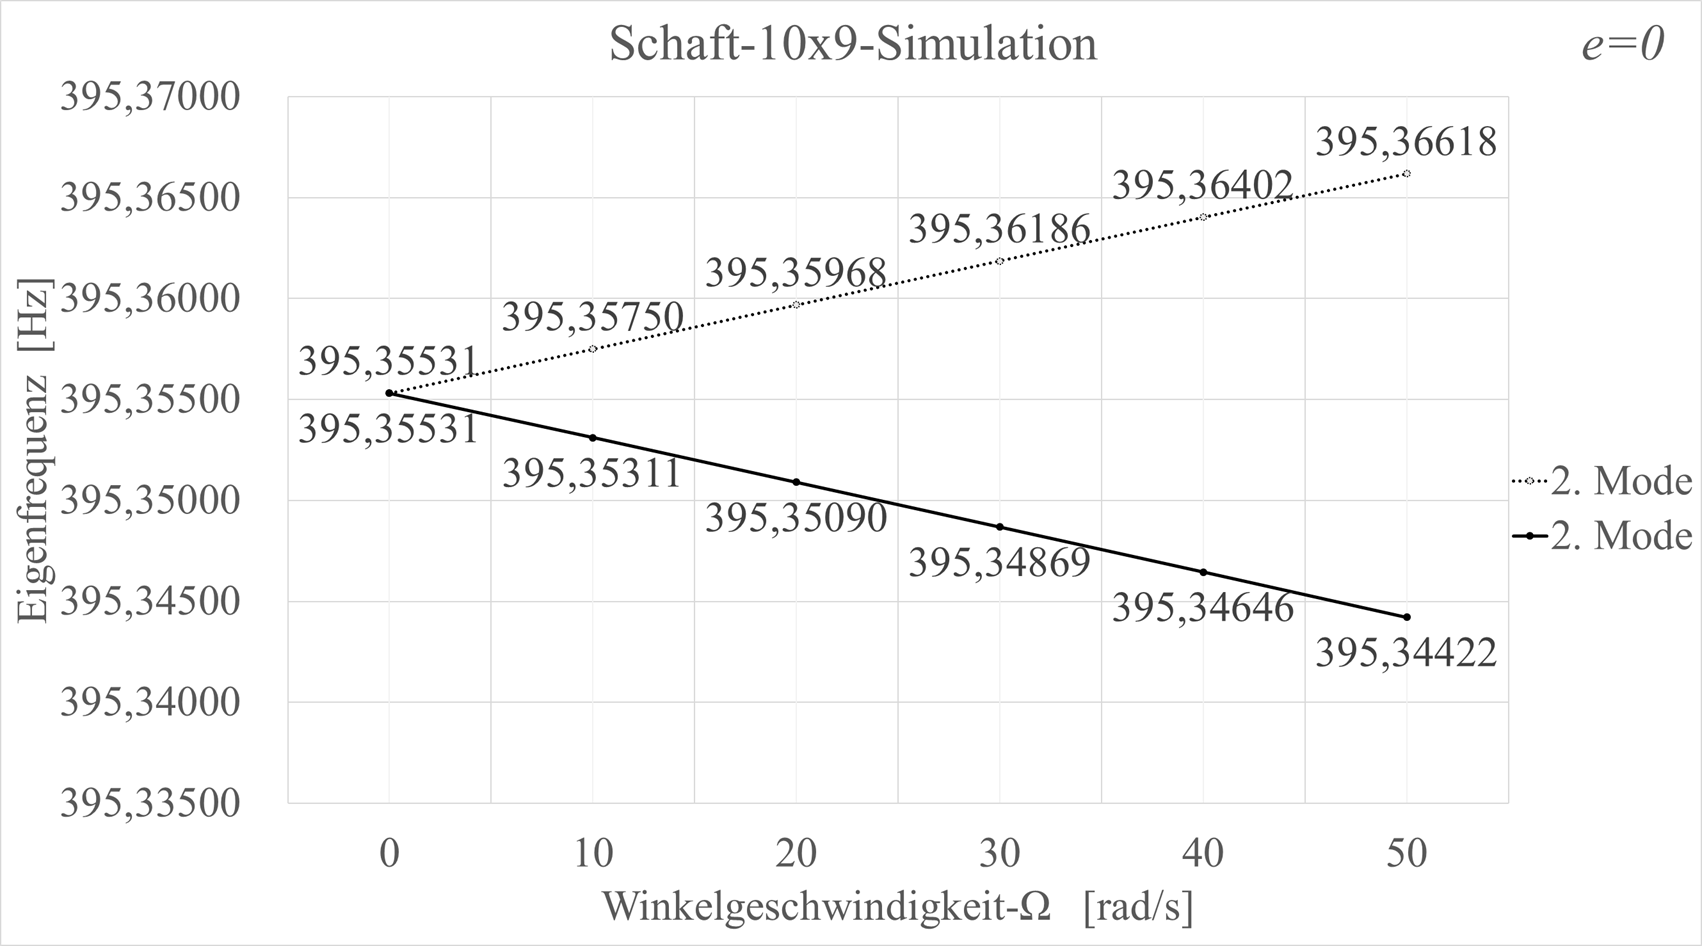
\includegraphics[width=0.95\linewidth, height=0.36\textheight]{Ergebnisse/Schaft_10x9_2Mode_Simu_ruhend}
		\caption{Eigenfrequenzen vom 2. Biegemode in Abhängigkeit der Winkelgeschwindigkeit bei einem Exzentrizitätsfehler von $ e=0 $ im ruhenden Inertialsystem. Berechnungsparameter: Schaft $ 10\times9 $, $\rho = 7800 \,\text{kg}/\text{m}^{3} $, $ E=2,1\cdot 10^{11} \,\text{N}/\text{m}^{2} $, $ \nu=0,28 $.}
		\label{fig:Result-Schaft-10x9-Simulation-2-Mode-ruhend}
	\end{figure}

	\begin{figure}[H]
		\centering
		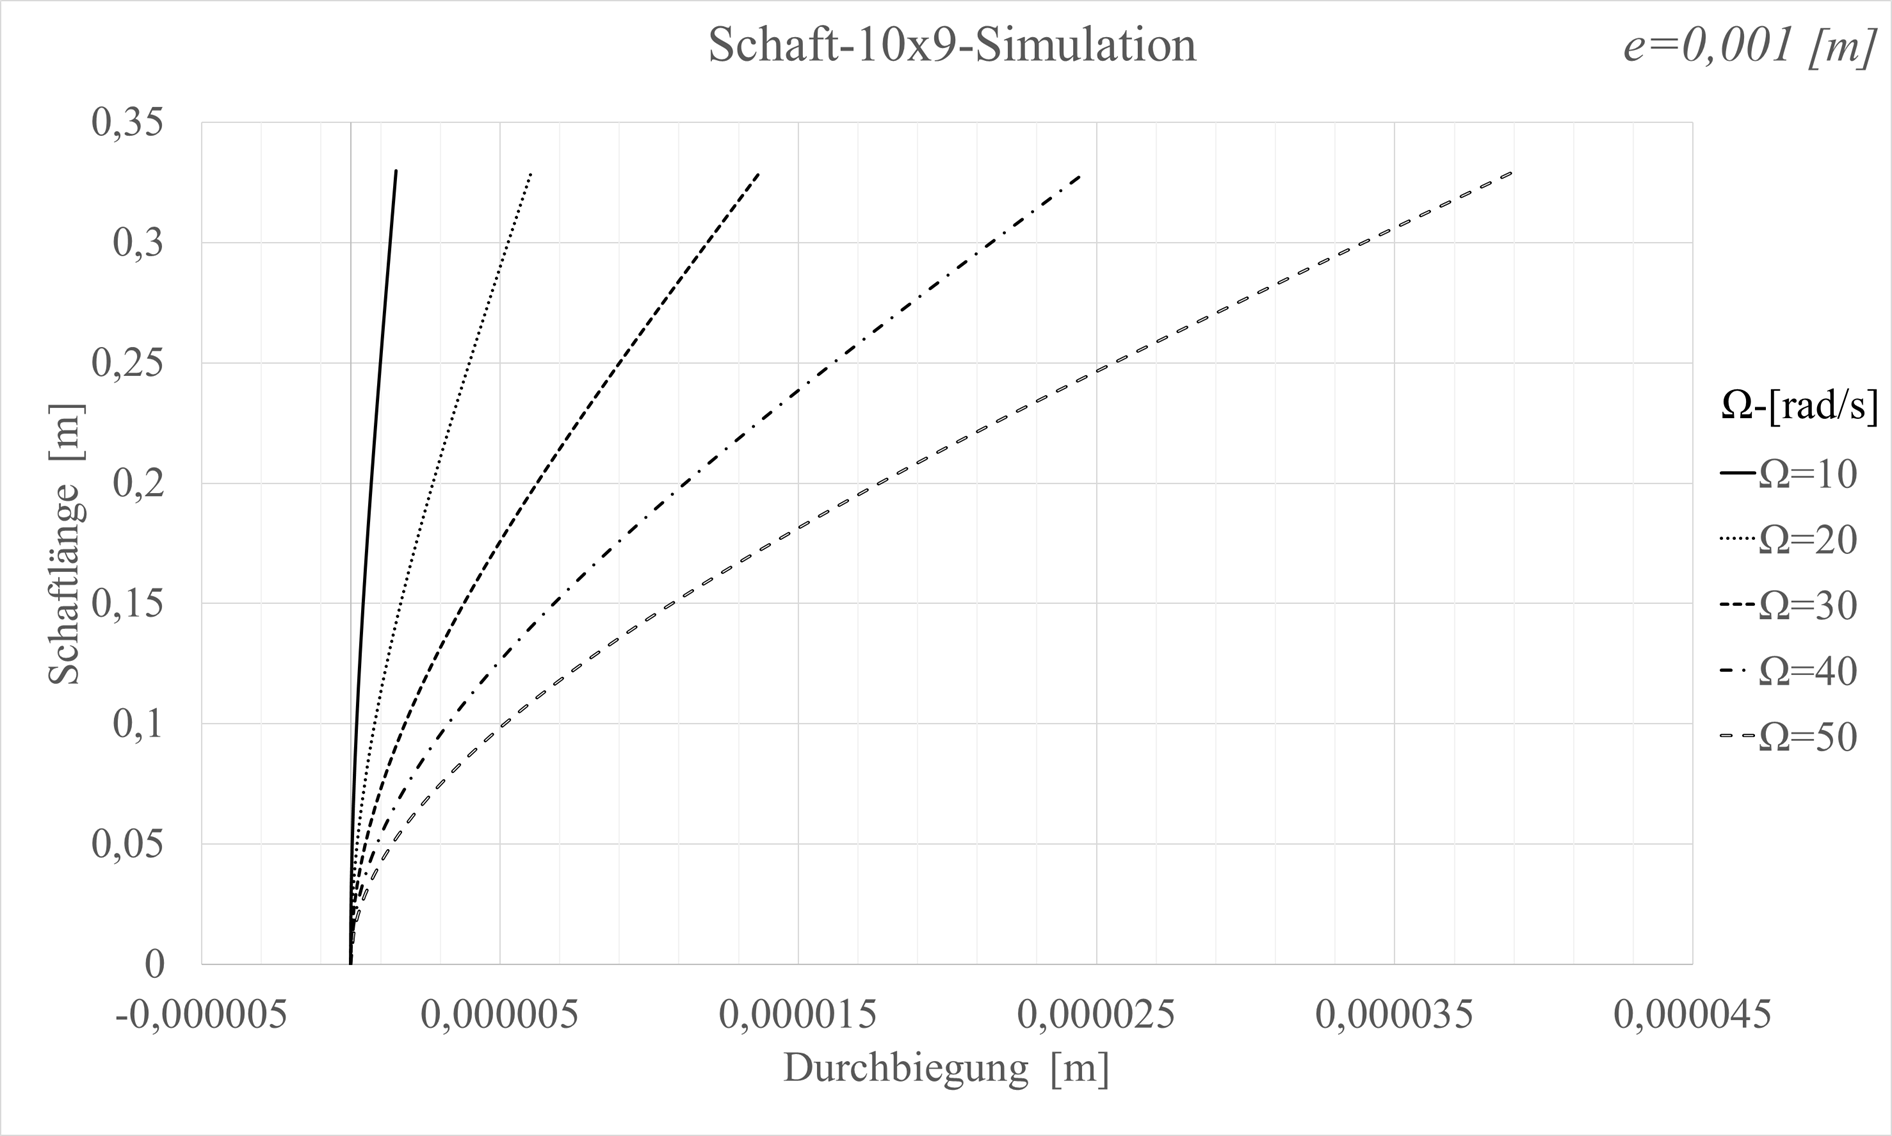
\includegraphics[width=0.95\linewidth, height=0.40\textheight]{Ergebnisse/Schaft_10x9_Biegung_Simu} 
		\caption{Durchbiegung in Abhängigkeit der Winkelgeschwindigkeit bei einem Exzentrizitätsfehler von $ e=0,001\,\text{m}$. Berechnungsparameter: Schaft $ 10\times9 $, $\rho = 7800 \,\text{kg}/\text{m}^{3} $, $ E=2,1\cdot 10^{11} \,\text{N}/\text{m}^{2} $, $ \nu=0,28 $.}
		\label{fig:Result-Schaft-10x9-Simulation-Durchbiegung}
	\end{figure}
	
	
	\begin{figure}[H]
		\centering
		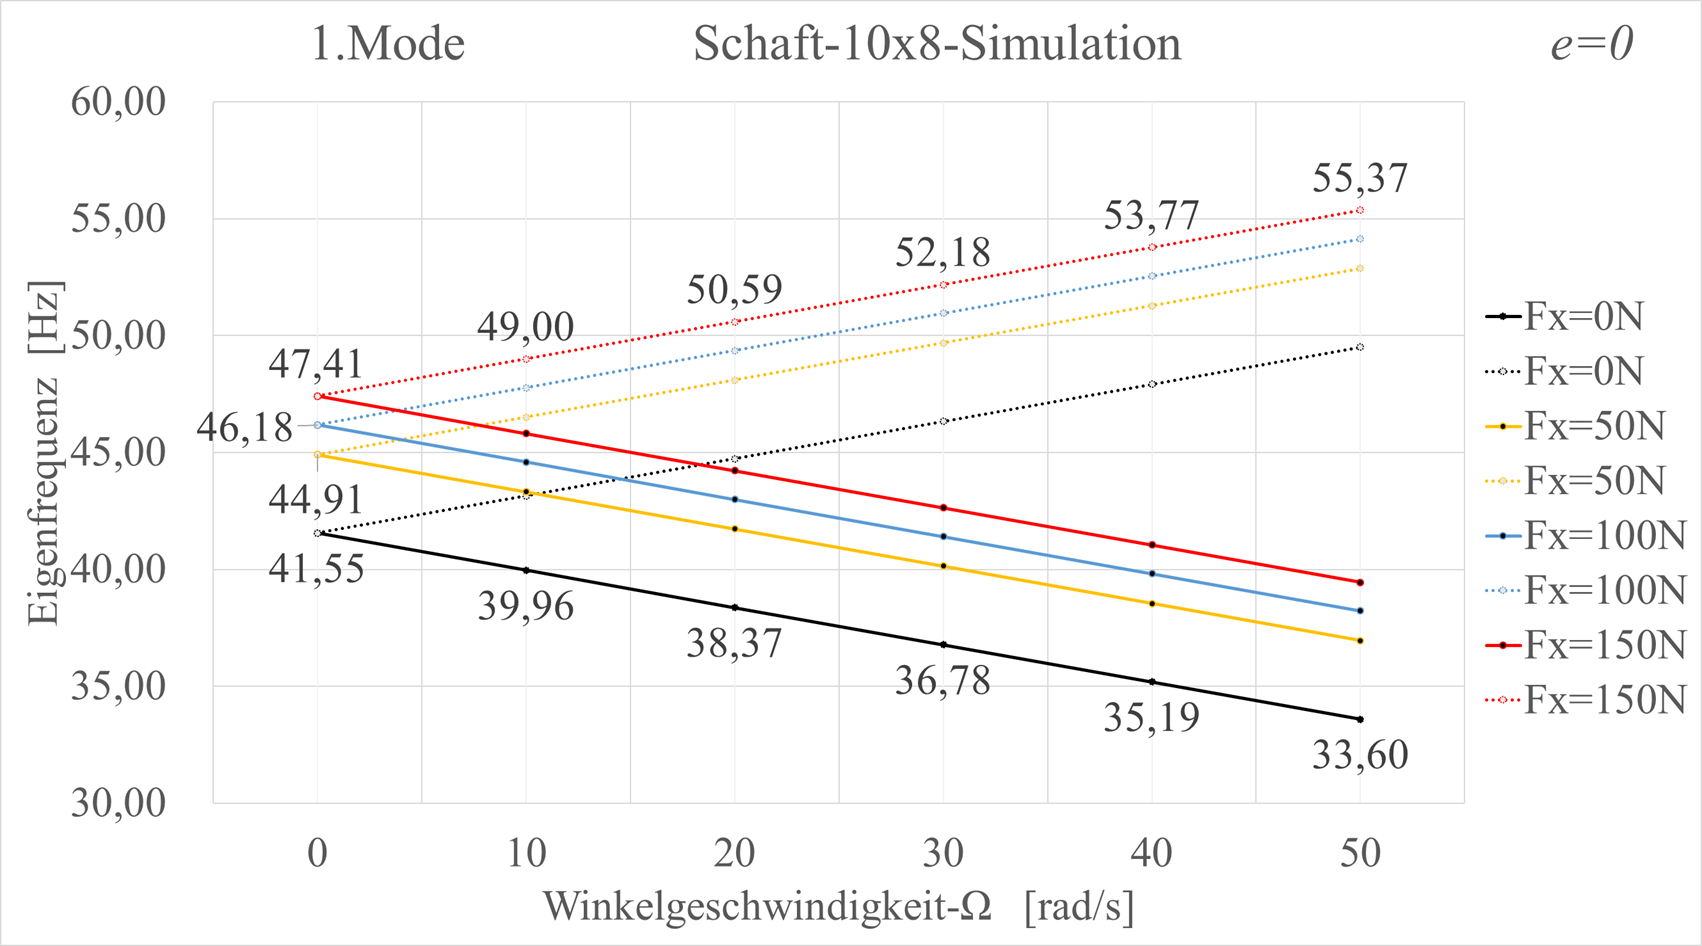
\includegraphics[width=0.95\linewidth, height=0.38\textheight]{Ergebnisse/Schaft_10x9_Zugkraft_Simu} 
		\caption{Eigenfrequenzen vom 1. Biegemode in Abhängigkeit der Winkelgeschwindigkeit $ \Omega $ und der Zugkraft $ Fx $ bei einem Exzentrizitätsfehler von $ e=0 $. Berechnungsparameter: Schaft $ 10\times9 $, $\rho = 7800 \,\text{kg}/\text{m}^{3} $, $ E=2,1\cdot 10^{11} \,\text{N}/\text{m}^{2} $, $ \nu=0,28 $.}
		\label{fig:Result-Schaft-10x9-Simulation-Zugkraft}
	\end{figure}


	
	\begin{figure}[H]
		\centering
		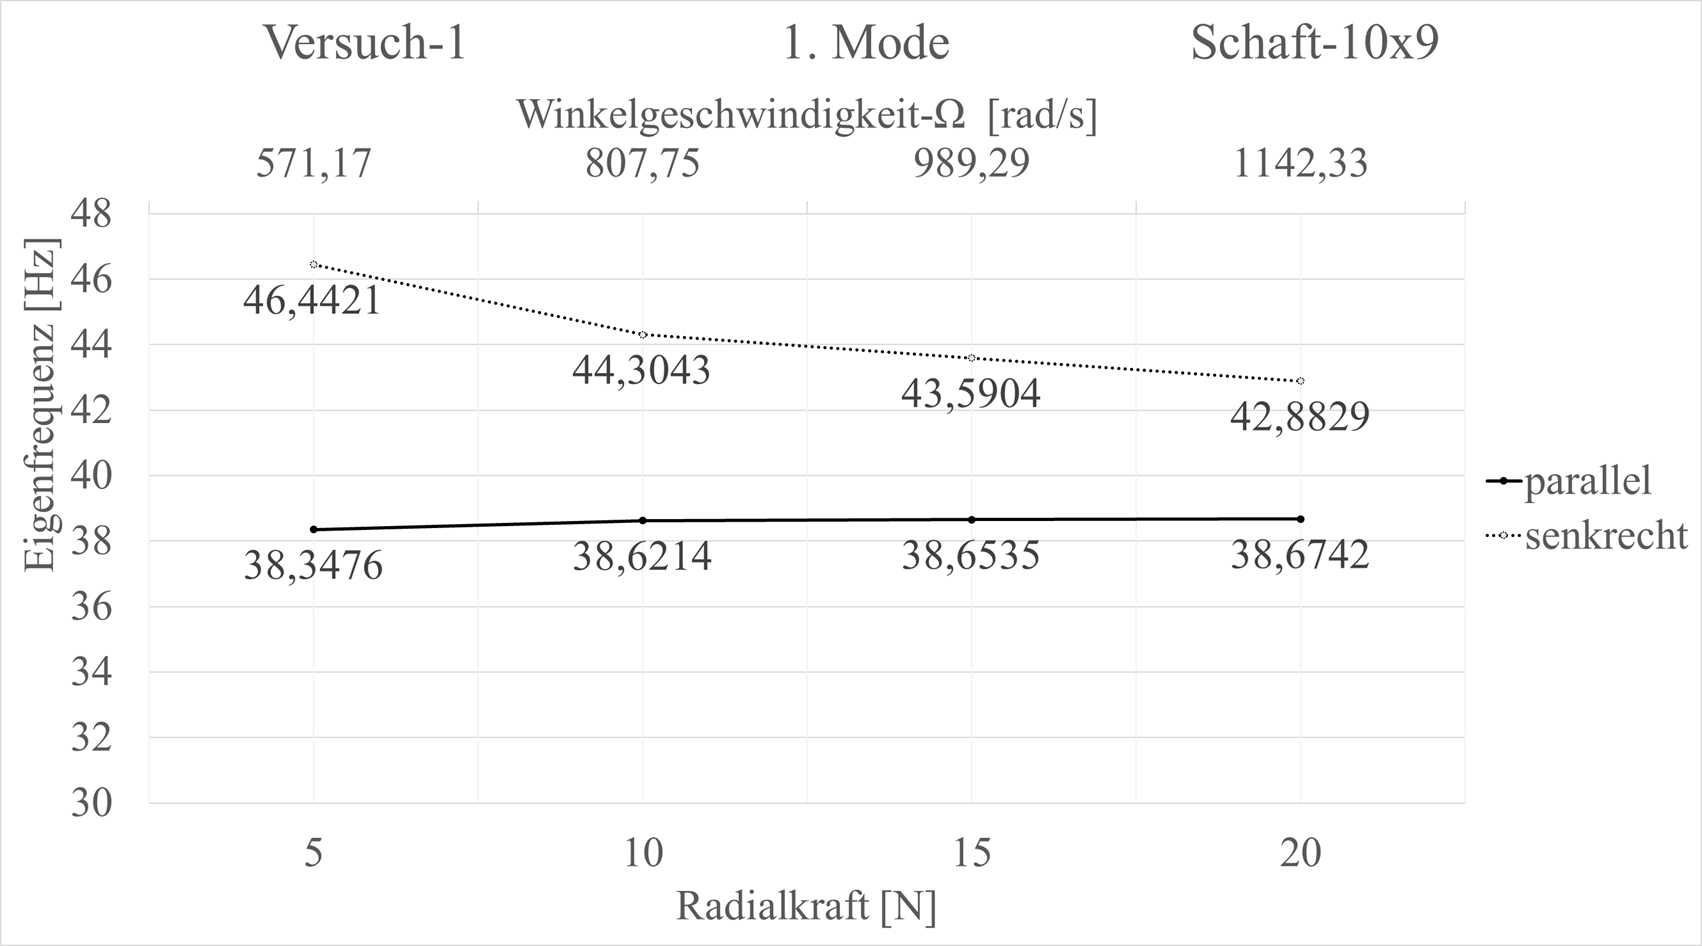
\includegraphics[width=0.95\linewidth, height=0.36\textheight]{Ergebnisse/Schaft_10x9_1Mode_ver1} 
		\caption{Gemessene Eigenfrequenzen vom 1. Biegemode in Abhängigkeit der Vorspannkraft. Angabe der Eigenfrequenzen parallel und senkrecht zur Vorspannrichtung (Probe Nr. 1 (Schaft $ 10\times9 $ ), Versuchsreihe 1).}
		\label{fig:Result-Schaft-10x9-1Mode-Ver1}
	\end{figure}
	
	\begin{figure}[H]
		\centering
		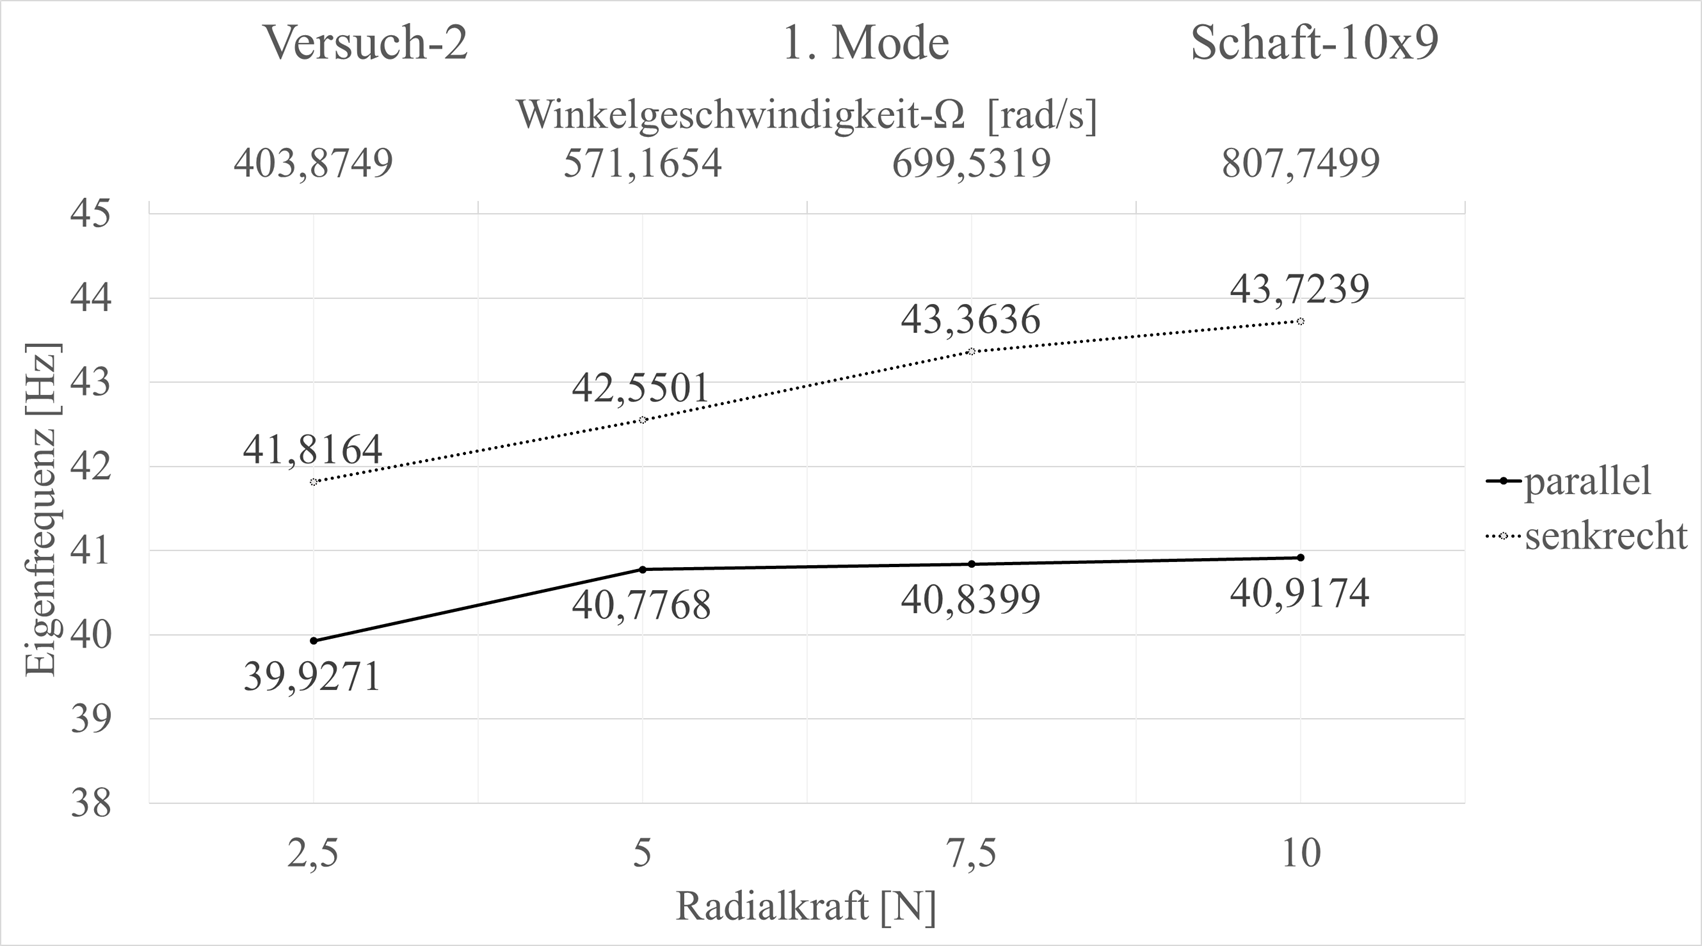
\includegraphics[width=0.95\linewidth, height=0.36\textheight]{Ergebnisse/Schaft_10x9_1Mode_ver2} 
		\caption{Gemessene Eigenfrequenzen vom 1. Biegemode in Abhängigkeit der Vorspannkraft. Angabe der Eigenfrequenzen parallel und senkrecht zur Vorspannrichtung (Probe Nr. 1 (Schaft $ 10\times9 $ ), Versuchsreihe 2).}
		\label{fig:Result-Schaft-10x9-1Mode-Ver2}
	\end{figure}

	\begin{figure}[H]
		\centering
		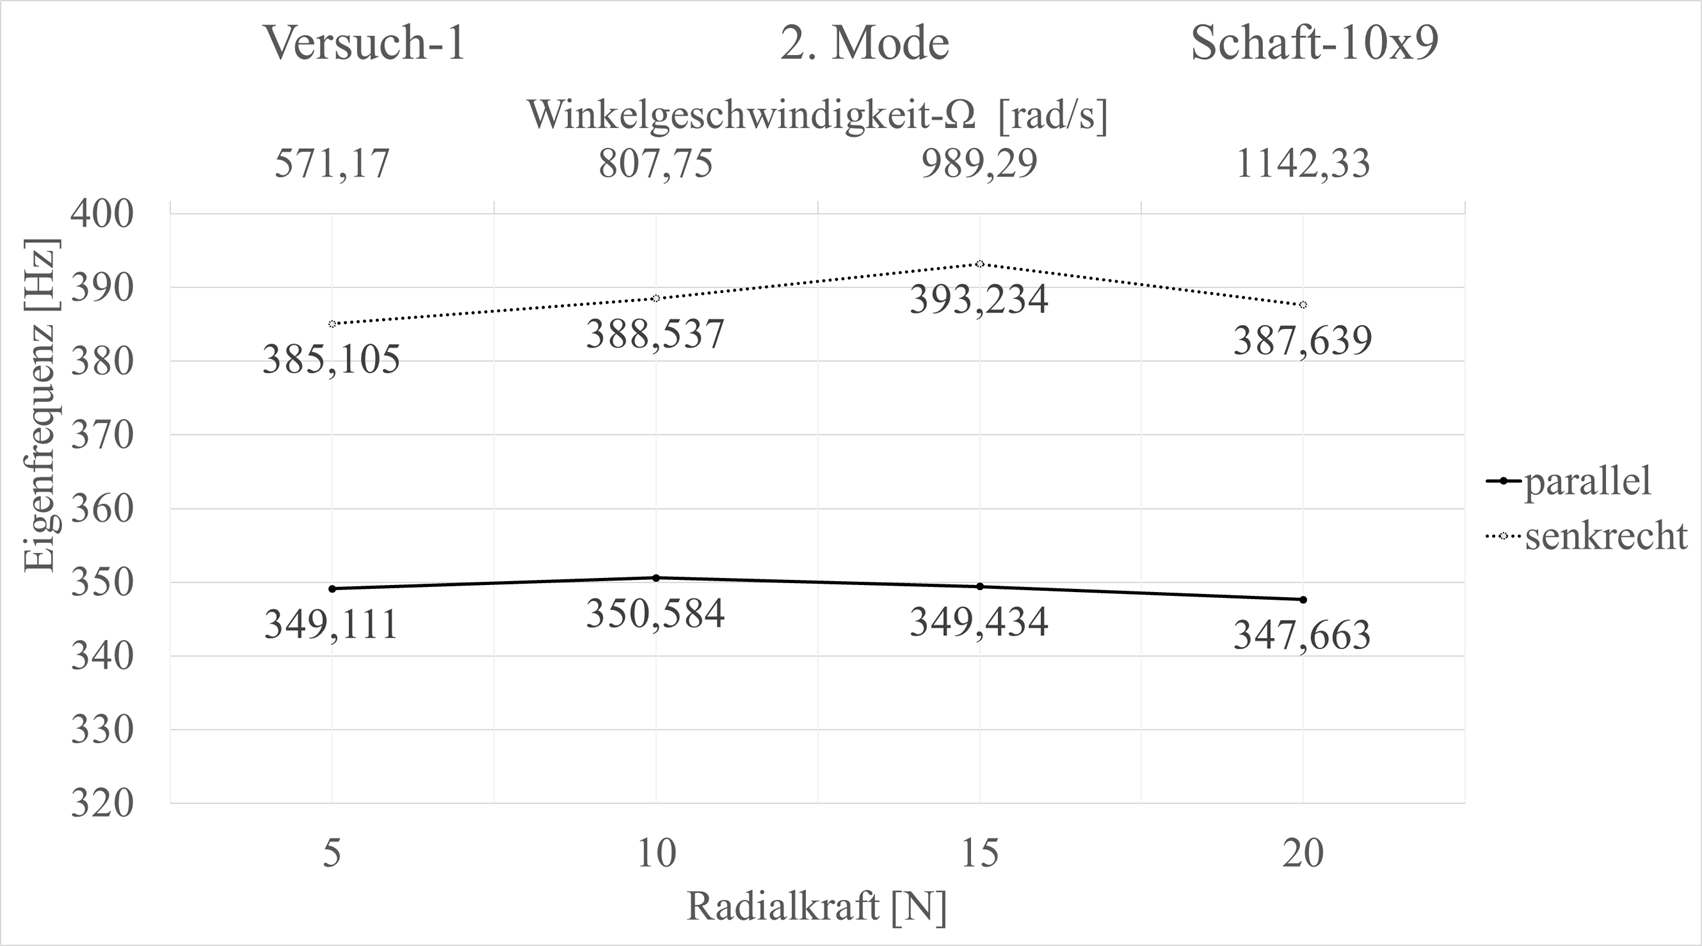
\includegraphics[width=0.95\linewidth, height=0.36\textheight]{Ergebnisse/Schaft_10x9_2Mode_ver1} 
		\caption{Gemessene Eigenfrequenzen vom 2. Biegemode in Abhängigkeit der Vorspannkraft. Angabe der Eigenfrequenzen parallel und senkrecht zur Vorspannrichtung (Probe Nr. 1 (Schaft $ 10\times9 $ ), Versuchsreihe 1).}
		\label{fig:Result-Schaft-10x9-2Mode-Ver1}
	\end{figure}

	\begin{figure}[H]
		\centering
		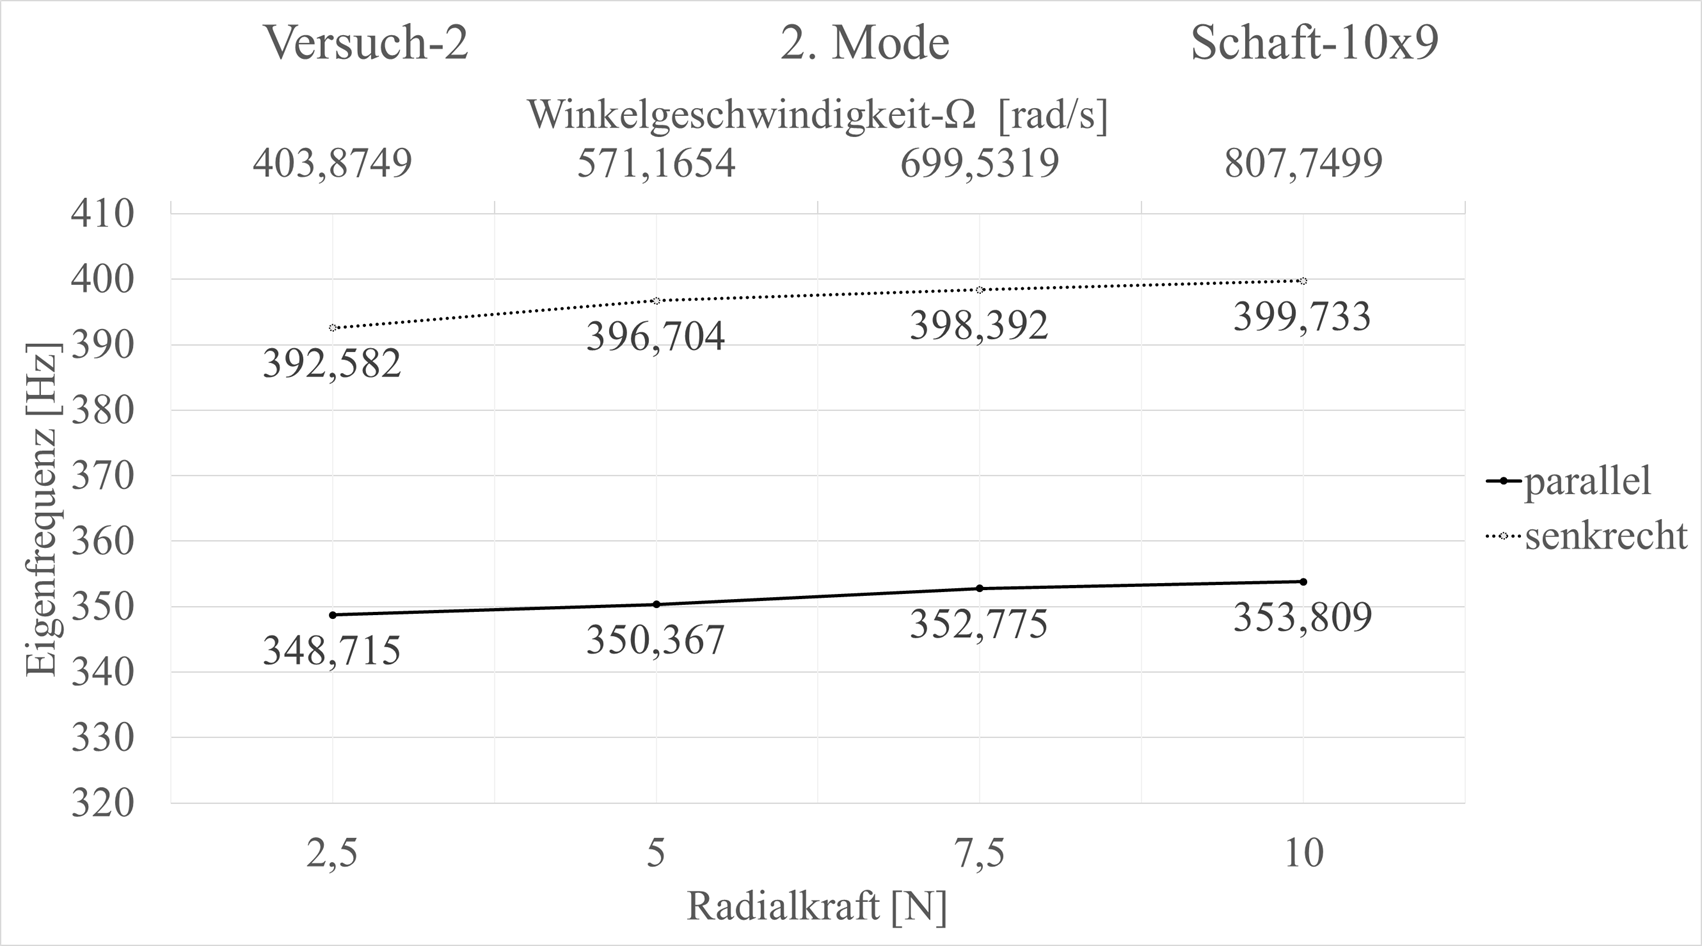
\includegraphics[width=0.95\linewidth, height=0.36\textheight]{Ergebnisse/Schaft_10x9_2Mode_ver2} 
		\caption{Gemessene Eigenfrequenzen vom 2. Biegemode in Abhängigkeit der Vorspannkraft. Angabe der Eigenfrequenzen parallel und senkrecht zur Vorspannrichtung (Probe Nr. 1 (Schaft $ 10\times9 $ ), Versuchsreihe 2).}
		\label{fig:Result-Schaft-10x9-2Mode-Ver2}
	\end{figure}

	 Der Einfluss der Vorspannkraft auf die Eigenfrequenzen ist ähnlich wie bei Probe 1. Die in den Abbildungen gezeigte Winkelgeschwindigkeit wurde wieder, mit einem konstanten Exzentrizitätsfehler von $ e=0,001\,\text{m}$, nach \ref{equ:Verhältnis-Rotaion-und-Radialkraft} berechnet. \\
	 Für den ersten Mode kann erneut eine tendenzielle Versteifung der Eigenfrequenzen festgestellt werden, wobei der Einfluss senkrecht zur Vorspannrichtung größer ist als parallel dazu. Gleiches gilt auch für die Eigenfrequenzen von Mode 2. Der relative Einfluss ist hier jedoch geringer.
	 Erneut sind die simulierten Eigenfrequenzen des ruhenden Schaft etwas höher als die gemessenen Werte. 
	 \\
	 Es ist ersichtlich, dass die experimentellen Ergebnisse eine gewisse Zufälligkeit aufweisen. Um genauere Ergebnisse zu erhalten müssten mehrere Messungen durchgeführt und diese dann gemittelt werden.
	
	